\documentclass[unknownkeysallowed]{beamer}
\mode<presentation>
{
%  \usetheme{AnnArbor}
%  \usetheme{Dresden}
%  \usetheme{Montpellier}
%  \usetheme{Antibes}
%  \usetheme{Frankfurt}
%  \usetheme{PaloAlto}
%  \usetheme{Bergen}
%  \usetheme{Boadilla}
%  \usetheme{Goettingen}
%  \usetheme{Pittsburgh}	%!!
%  \usetheme{Berkeley}
%  \usetheme{Hannover}
%  \usetheme{Rochester}		%!!!
%  \usetheme{Berlin}
%  \usetheme{Ilmenau}
%  \usetheme{Singapore}
  \usetheme{Boadilla}		%viel platz
%  \usetheme{JuanLesPins}
%  \usetheme{Szeged}		%!
%  \usetheme{boxes}
%  \usetheme{Luebeck}
%  \usetheme{Warsaw}
%  \usetheme{Copenhagen}
%  \usetheme{Madrid}
%  \usetheme{Darmstadt}
%  \usetheme{Malmoe}
%  \usetheme{default}
%  \usetheme{JuanLesPins}

%  \usetheme{Marburg}


%\usefonttheme{professionalfonts}
%	default | professionalfonts | serif |
%	structurebold | structureitalicserif |
%	structuresmallcapsserif
%\useinnertheme{rounded}
%	circles | default | inmargin |
%	rectangles | rounded

%  \setbeamercovered{transparent}
  % oder auch nicht
\usecolortheme{rose}


\definecolor{uaf yellow}{cmyk}{0,0.16,1,0} % official UAF yellow
\definecolor{light yellow}{cmyk}{0.01,0,0.16,0}
\definecolor{uaf blue}{cmyk}{1,0.66,0,0.02} % official UAF blue
\definecolor{light blue}{cmyk}{0.22,0.11,0,0}
\definecolor{arsc blue}{HTML}{005496}
\definecolor{arsc red}{HTML}{a20a42}
\definecolor{arsc green}{HTML}{009a82}
\definecolor{light gray}{HTML}{777777}

  %navigation aus, klaut nur platz
  \setbeamertemplate{navigation symbols}{}
% Reset title background to default
%\setbeamertemplate{title page}[default]
\setbeamercolor{title}{bg=}
\setbeamercolor{frametitle}{bg=uaf blue, fg=white}
\setbeamercolor{institute}{fg=white}
\setbeamercolor{date}{fg=white}
\setbeamercolor{block}{bg=}
%\setbeamercolor{title}{fg=black}

% Reset block background to default
%\setbeamertemplate{blocks}[default]
%\setbeamercolor{block title}{bg=}
%\setbeamercolor{block body}{bg=}

\beamertemplatenavigationsymbolsempty  
\setbeamertemplate{blocks}[rounded][shadows=false]

\useinnertheme{circles}

}
\usepackage[latin1]{inputenc}
\usepackage{latexsym}
\usepackage{amsfonts}
%\usepackage{natbib}
\usepackage{fancyhdr}
\usepackage{graphicx}
%\usepackage{subfigure}
% oder was auch immer
\usepackage{grffile}
\usepackage{pgf}
\usepackage{tikz}

\usepackage{listings}

\usepackage{times}
\usepackage[T1]{fontenc}
%\usepackage{appendixnumber}
% Oder was auch immer. Zu beachten ist, das Font und Encoding passen
% müssen. Falls T1 nicht funktioniert, kann man versuchen, die Zeile
% mit fontenc zu löschen.

\hypersetup{
    bookmarks=true,         % show bookmarks bar?
    unicode=false,          % non-Latin characters in Acrobat's bookmarks
    pdftoolbar=true,        % show Acrobat's toolbar?
    pdfmenubar=true,        % show Acrobat's menu?
    pdffitwindow=false,     % window fit to page when opened
    pdfstartview={FitH},    % fits the width of the page to the window
    pdftitle={My title},    % title
    pdfauthor={Author},     % author
    pdfsubject={Subject},   % subject of the document
    pdfcreator={Creator},   % creator of the document
    pdfproducer={Producer}, % producer of the document
    pdfkeywords={keyword1} {key2} {key3}, % list of keywords
    pdfnewwindow=true,      % links in new window
    colorlinks=false,       % false: boxed links; true: colored links
    linkcolor=red,          % color of internal links
    citecolor=green,        % color of links to bibliography
    filecolor=magenta,      % color of file links
    urlcolor=cyan           % color of external links
}

\title[PAG]% (optional, nur bei langen Titeln nötig)
{GEOS 436 / 636\\
Programming and Automation for Geoscientists\\[20pt]
-- Week 12: Generic Mapping Tools I --
}

\author[Grapenthin]% (optional, nur bei vielen Autoren)
{Ronni Grapenthin\\
rgrapenthin@alaska.edu\\
Elvey 413B\\
x7682}
% - Namen müssen in derselben Reihenfolge wie im Papier erscheinen.
% - Der \inst{?} Befehl sollte nur verwendet werden, wenn die Autoren
%   unterschiedlichen Instituten angehören.

\institute[UAF] % (optional, aber oft nötig)
{}
% - Der \inst{?} Befehl sollte nur verwendet werden, wenn die Autoren
%   unterschiedlichen Instituten angehören.
% - Keep it simple, niemand interessiert sich für die genau Adresse.

% - Namen müssen in derselben Reihenfolge wie im Papier erscheinen.
% - Der \inst{?} Befehl sollte nur verwendet werden, wenn die Autoren
%   unterschiedlichen Instituten angehören.

% - Der \inst{?} Befehl sollte nur verwendet werden, wenn die Autoren
%   unterschiedlichen Instituten angehören.
% - Keep it simple, niemand interessiert sich für die genau Adresse.

\date[]{}

% - Volle oder abgekürzter Name sind möglich.
% - Dieser Eintrag ist nicht für das Publikum gedacht (das weiß
%   nämlich, bei welcher Konferenz es ist), sondern für Leute, die diese
%   Folien später lesen.

%\AtBeginSection[]
%{
%  \begin{frame}<beamer>
%    \frametitle{Outline}
%    \tableofcontents[currentsection,currentsubsection]
%  \end{frame}
%}

% Falls Aufzählungen immer schrittweise gezeigt werden sollen, kann
% folgendes Kommando benutzt werden:

%\beamerdefaultoverlayspecification{<+->}

%%switch on to have only frame numbers
\setbeamertemplate{footline}[frame number]

\defbeamertemplate*{title page}{customized}[1][]
{
		\begin{tikzpicture}
			\node[text width=\textwidth,
				fill=gray!70, 
				fill opacity=0.75,
				text opacity=1,
				rounded corners = 10pt,
				inner sep=2pt]{
				\begin{center}	
			  \usebeamerfont{title}{\bf \usebeamercolor[fg]{title} \inserttitle}
			  \par
			  \usebeamerfont{subtitle}\insertsubtitle\par
			  \bigskip
			  \usebeamerfont{author}\insertauthor\par
			  \bigskip
			  \usebeamerfont{institute}\insertinstitute\par
			  \bigskip
			  \usebeamerfont{date}\insertdate\par
			  \end{center}
			  };
	\end{tikzpicture}		  
%	\vspace{0.4cm}\usebeamercolor[fg]{titlegraphic}\inserttitlegraphic 
%	\begin{flushright}
%	\vspace{-1.25cm}\includegraphics[width=2cm]{../moore_logo_transp.png}\vspace{5cm}
%	\end{flushright}
}

\begin{document}

\lstset{numbers=left, numberstyle=\tiny, stepnumber=2, basicstyle=\ttfamily, numbersep=5pt, xleftmargin=10pt}

\setbeamertemplate{background}{\includegraphics[width=\paperwidth]{/home/roon/Pictures/rooftop_initial.jpg}}

	\begin{frame}
	\begin{center}
		\titlepage
	\end{center}
	\end{frame}

\setbeamertemplate{background}{}

\begin{frame}
\frametitle{}
%	\vspace{2cm}
	How to automate making publication-quality:

	\begin{itemize}
		\item maps,
		\item x-y plots, 
		\item animations 
	\end{itemize}

	using world class base data sets while having maximum flexibility regarding layout of your product?
\end{frame}


\begin{frame}
\frametitle{}
	\begin{center}
		
\includegraphics[width=.8\textwidth]{../figures/gmt-logo.png}	
	\end{center}
	\begin{flushright}
	\tiny{\emph{\url{https://www.generic-mapping-tools.org}}}
	\end{flushright}	
\end{frame}

\begin{frame}
\frametitle{What is GMT?}
	\vspace{-0.25cm}
	\begin{center}
		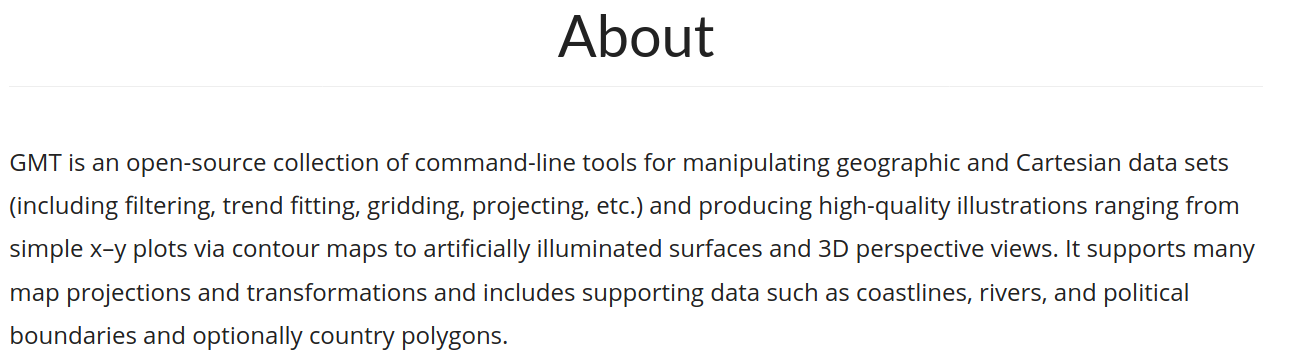
\includegraphics[width=\textwidth]{../figures/gmt_about.png}
	\end{center}
	\begin{flushright}
	\vspace{-0.15cm}
	\tiny{\emph{\url{https://www.generic-mapping-tools.org/about/}}}
	\end{flushright}	
\end{frame}

\begin{frame}
\frametitle{Make this with ONE command?}
	\begin{center}
		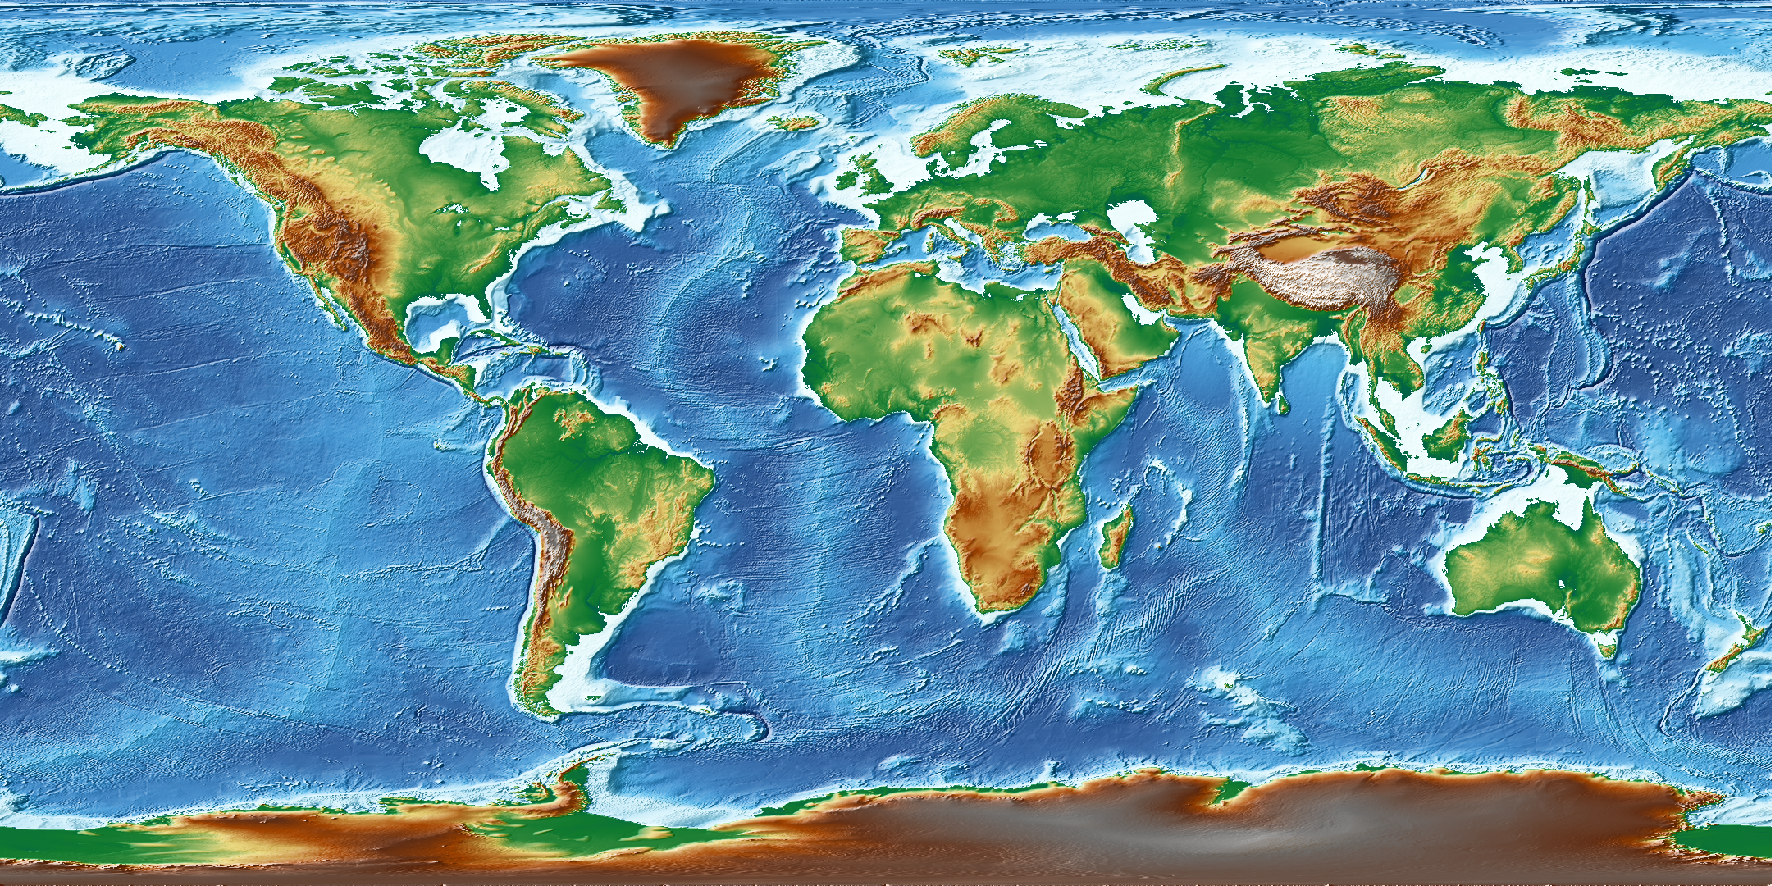
\includegraphics[width=\textwidth]{../figures/gmt_world_map.png}	
	\end{center}
\end{frame}

\begin{frame}[fragile=singleslide]
\frametitle{Make this with ONE command?}
	\begin{center}
		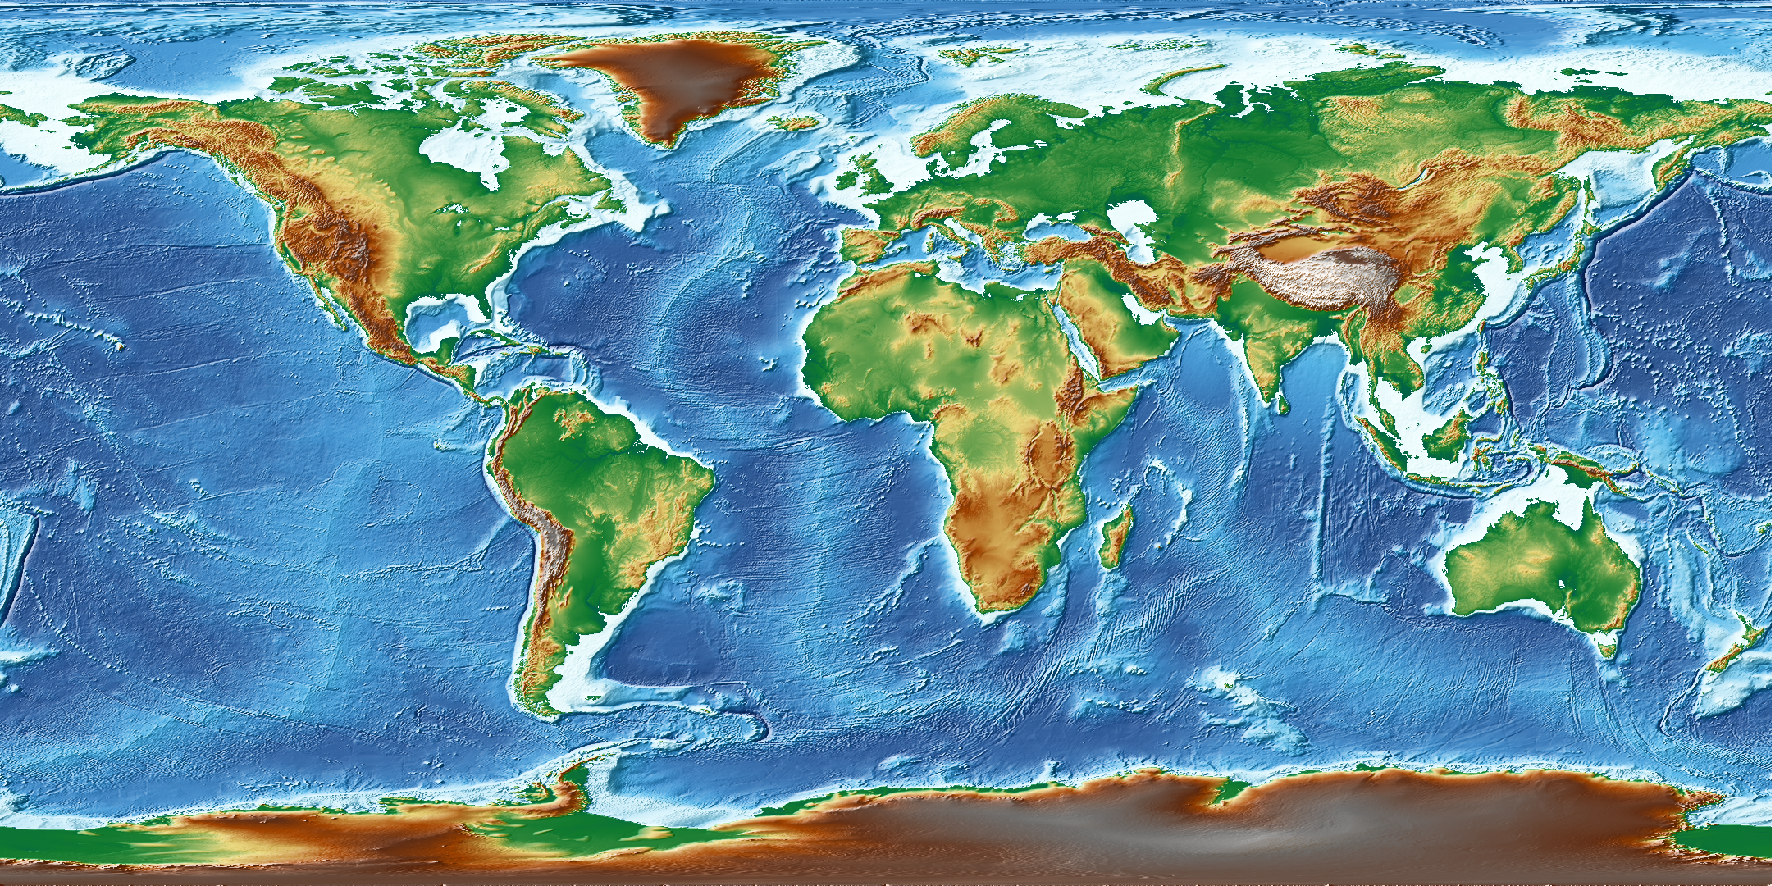
\includegraphics[width=\textwidth]{../figures/gmt_world_map.png}	
	\end{center}

	{\scriptsize	
	\begin{verbatim}
		$> gmt grdimage @earth_relief_10m -Rg -I+d -png world_map
	\end{verbatim}
	}
\end{frame}

\begin{frame}
\frametitle{What is GMT?}
	\vspace{-0.25cm}
	\begin{center}
		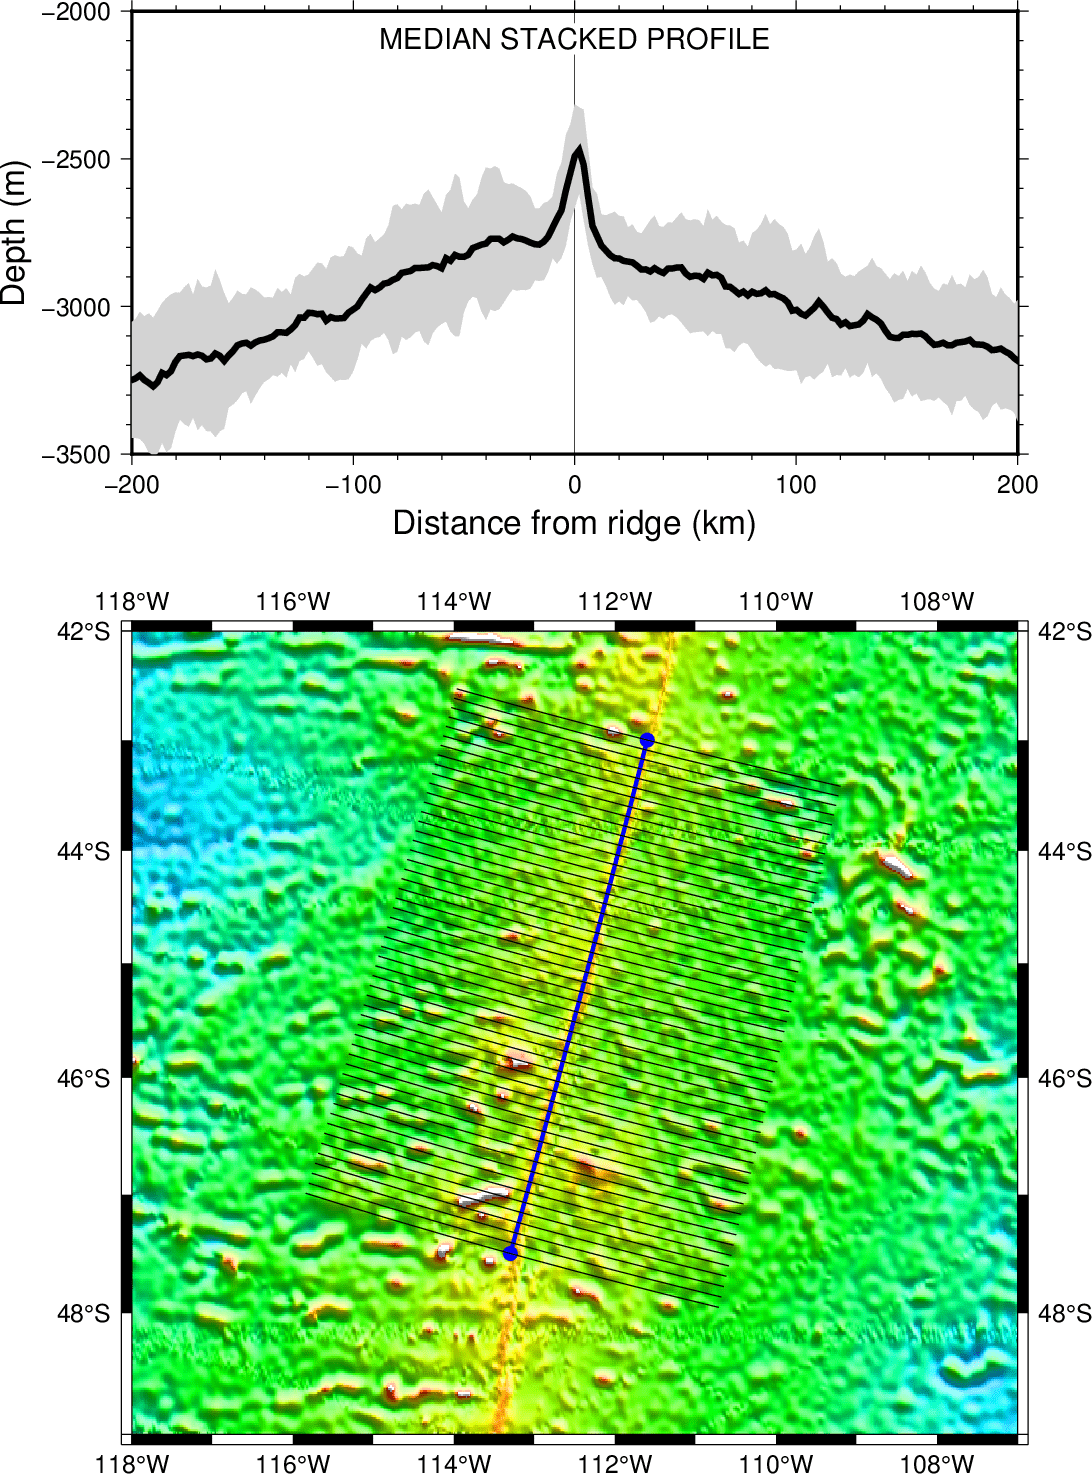
\includegraphics[width=.5\textwidth]{../figures/gmt_ex33.png}	
	\end{center}
	\begin{flushright}
	\vspace{-0.15cm}
	\tiny{\emph{\url{https://docs.generic-mapping-tools.org/latest/gallery/ex33.html}}}
	\end{flushright}	
\end{frame}

\begin{frame}
\frametitle{What is GMT?}
	Some history:
	\begin{itemize}
		\item Initiated in 1987 at Lamont-Doherty Earth Observatory by then graduate students Paul Wessel and Walter Smith
		\item Began as set of Unix command-line tools that generated PostScript
		\item Evolved to provide shell script, Matlab, and beginning Python and Julia support
	\end{itemize}
	\begin{center}
		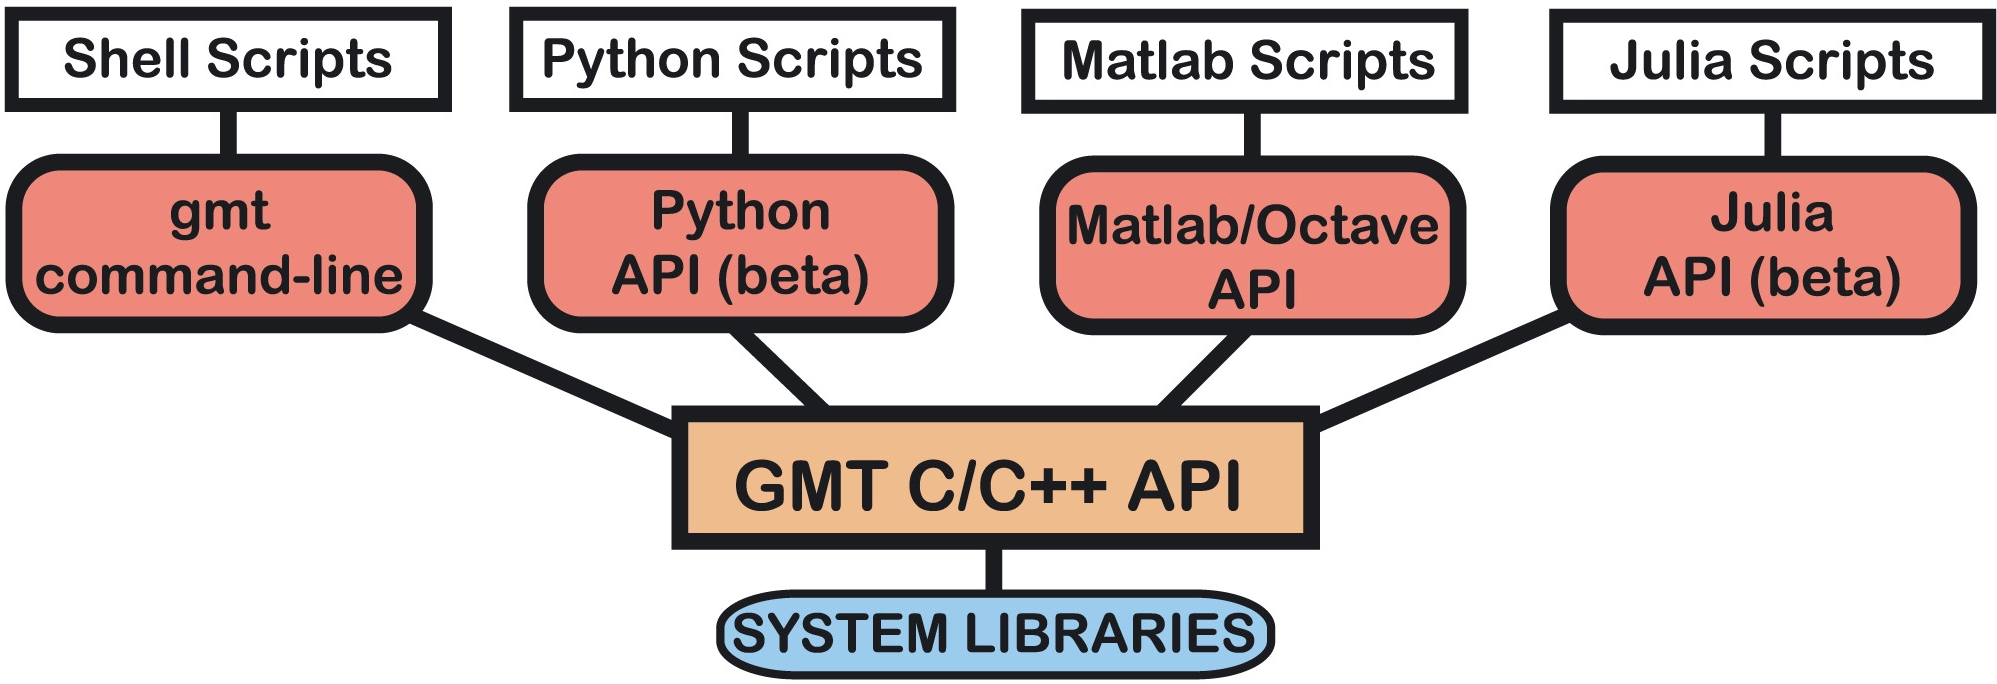
\includegraphics[width=.5\textwidth]{../figures/gmt_architecture.png}	
	\end{center}
	\begin{flushright}
	\tiny{\emph{Wessel et al., 2019}}
	\end{flushright}	
\end{frame}

\begin{frame}[fragile=singleslide]
\frametitle{GMT comes loaded}
	\begin{itemize}
		\item Includes GSHHG -- Global Self-consistent, Hierarchical, High-resolution Geography Database and DCW-GMT -- The Digital Chart of the World
		\begin{itemize}	
			\item coastlines
			\item national and state (for some countries) borders
			\item rivers / fresh-water bodies
		\end{itemize}
	\end{itemize}

	\begin{center}
		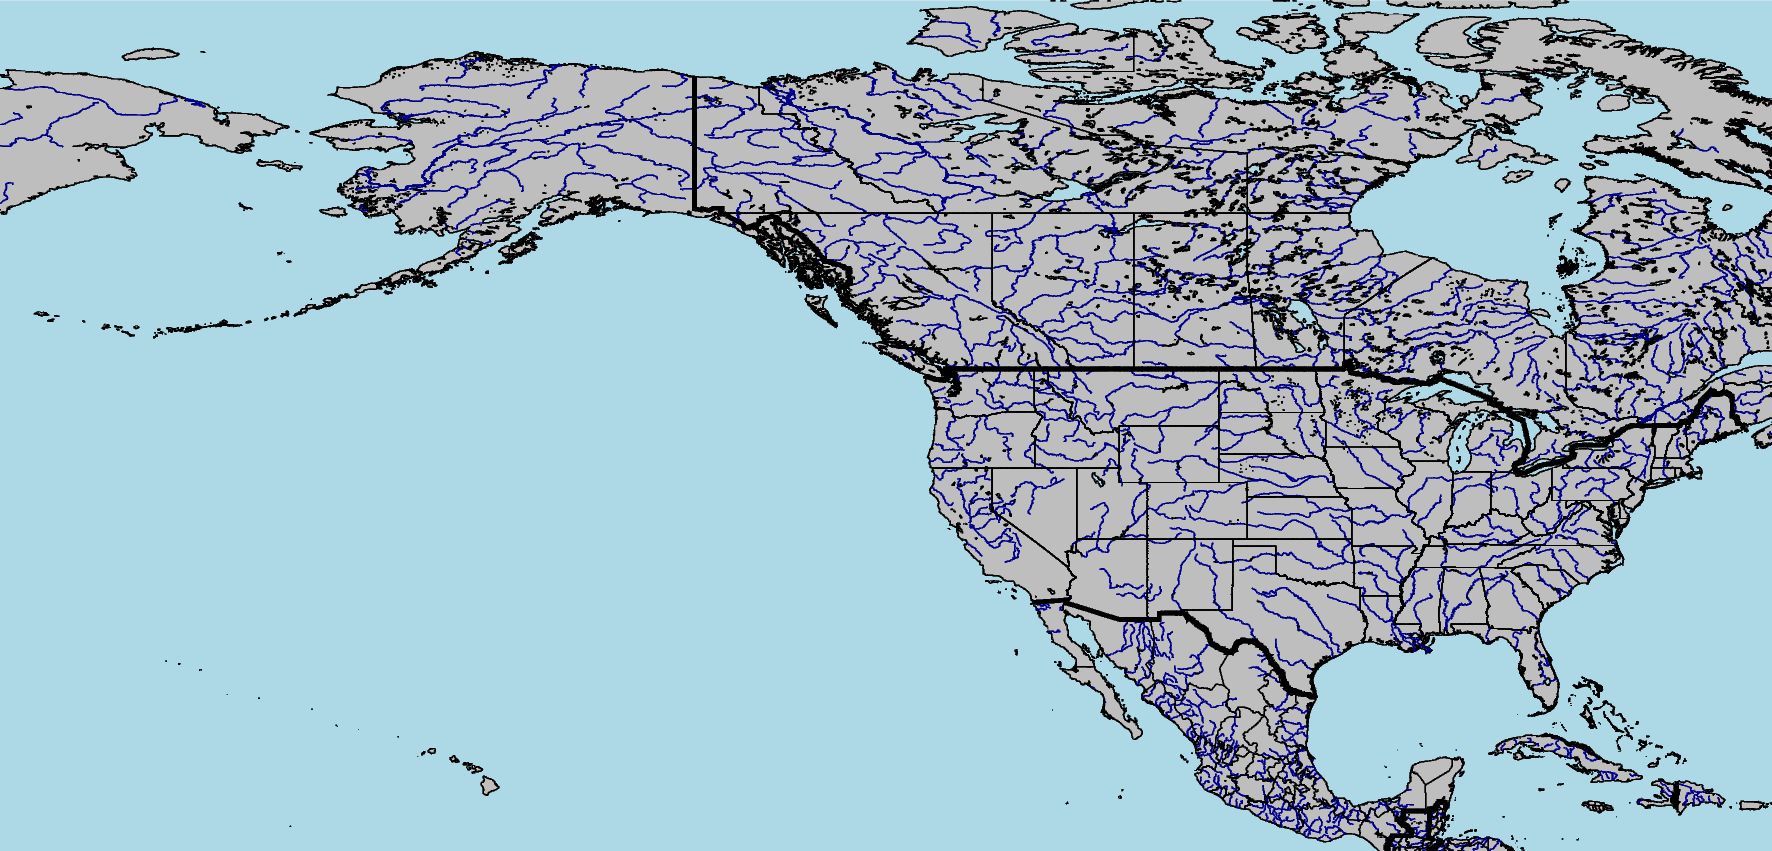
\includegraphics[width=0.75\textwidth]{../figures/gmt_coastlines.png}	
	\end{center}
	{\scriptsize	
	\begin{verbatim}
$> gmt coast -RUS+r5 -Ir/0.25p,darkblue \
             -N1/1p,black -N2/0.25p,black -W.25p,black \
             -Ggray -Slightblue -Df -png coastlines 
	\end{verbatim}
	}

\end{frame}

\begin{frame}[fragile=singleslide]
\frametitle{GMT comes loaded}
	\begin{itemize}
		\item Provides access to external data grids via remote file mechanism (will download file on first access then read locally)
		\begin{itemize}	
			\item Global Earth Relief Grids ({\tt earth\_relief})
			\item Global Earth Seafloor Crustal Age Grids ({\tt earth\_age})
			\item Global Earth Day/Night Images ({\tt earth\_day} and {\tt earth\_night})
			\item Global Earth Mask Grids ({\tt earth\_mask})
		\end{itemize}
		\item use default preferred color palette.
	\end{itemize}

	\begin{center}
			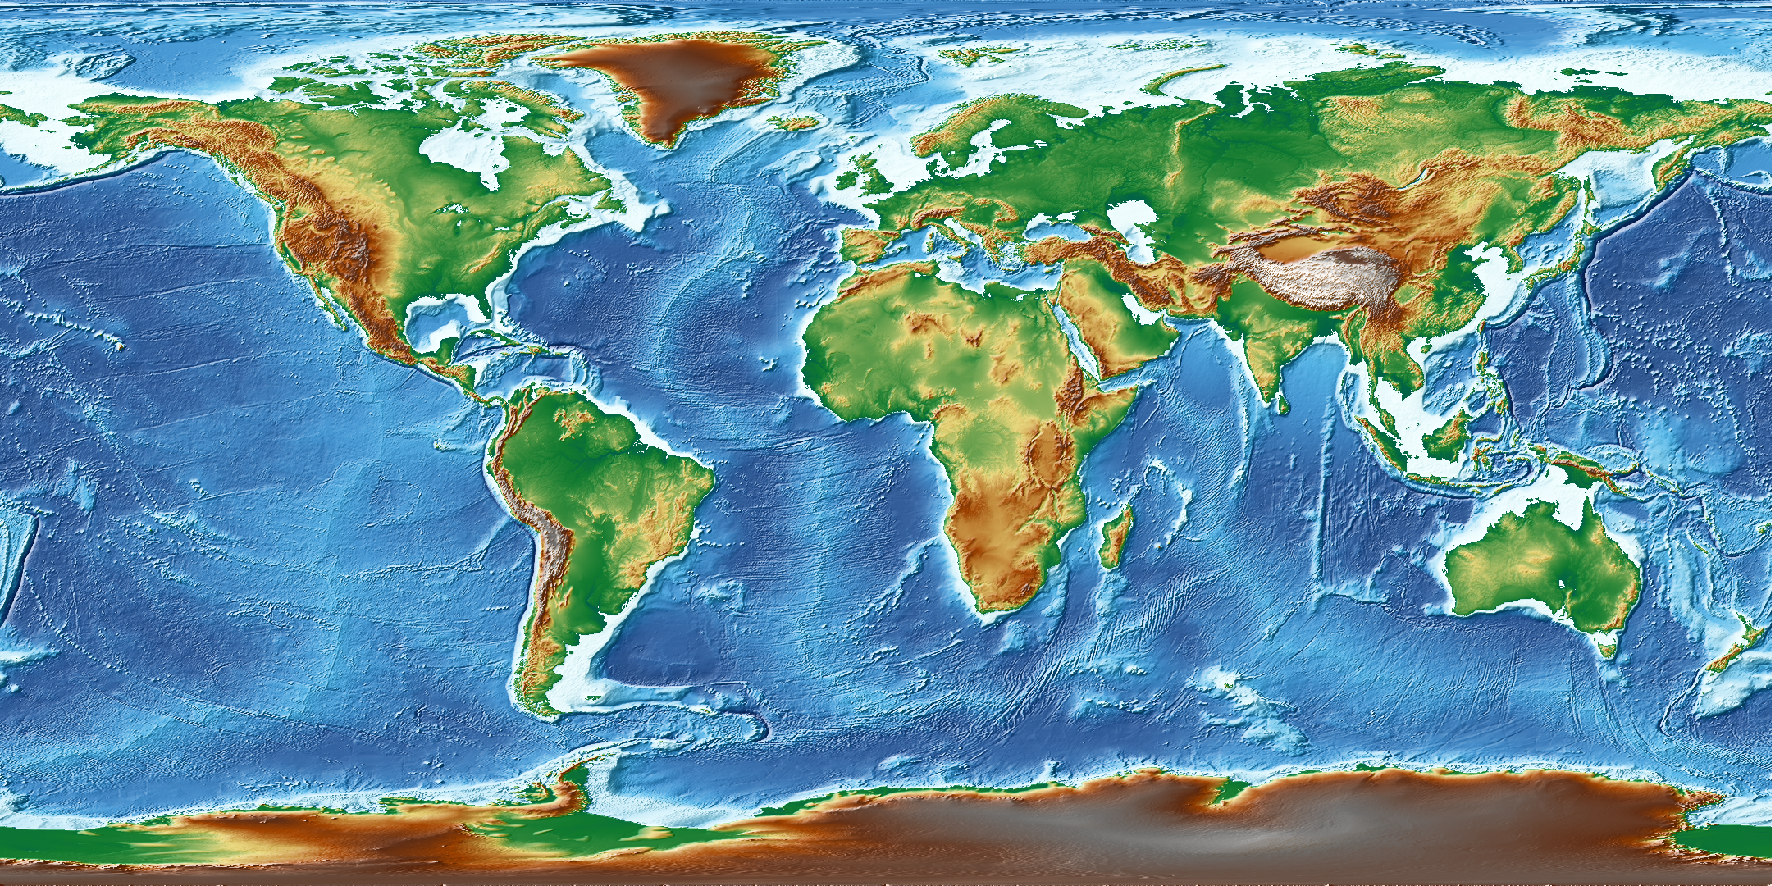
\includegraphics[width=0.48\textwidth]{../figures/gmt_world_map.png}	
			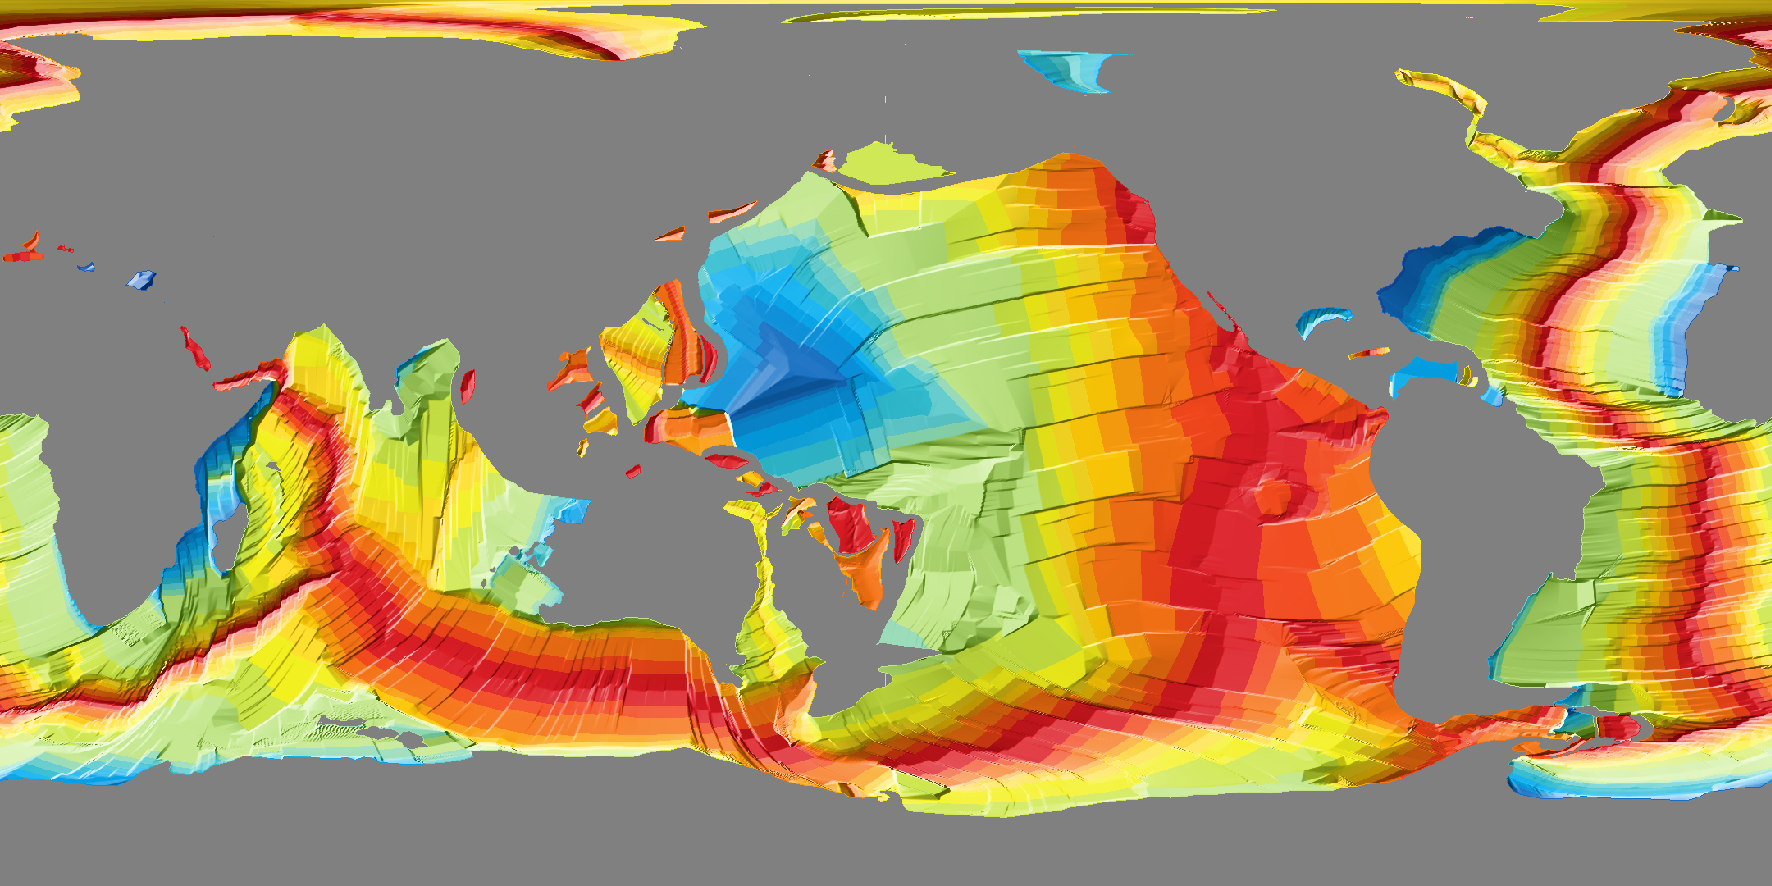
\includegraphics[width=0.48\textwidth]{../figures/gmt_world_map_age.png}	
	\end{center}
	{\scriptsize	
	\begin{verbatim}
$> gmt grdimage @earth_relief_10m -Rg -I+d -png world_map
$> gmt grdimage @earth_age_10m -Rg -I+d -png world_map_age
	\end{verbatim}
	}

\end{frame}

\begin{frame}
\frametitle{GMT comes loaded}
	\begin{itemize}
		\item More than 30 map projections to project globe onto flat paper, basic categories:
		\begin{itemize}	
			\item azimuthal/planar map projections (near poles)
			\item cylindrical map projections (near equator)
			\item conic map projections (in between)
			\item miscellaneous projections (xy plots, etc.)
		\end{itemize}
	\end{itemize}
	\begin{center}
			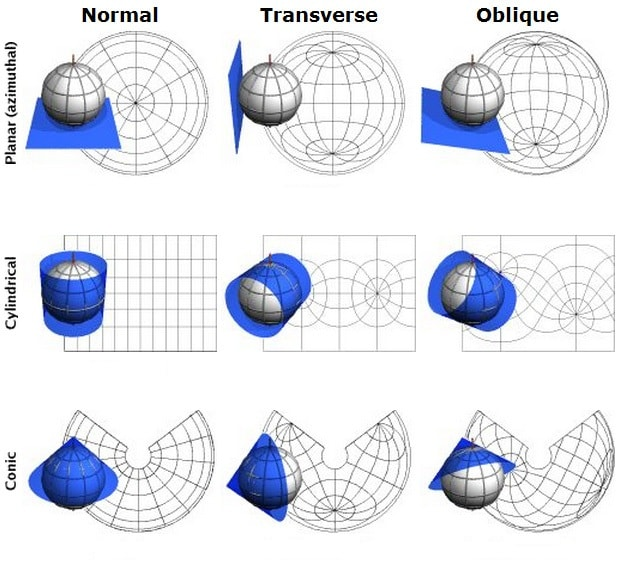
\includegraphics[width=0.48\textwidth]{../figures/map_projections.jpg}	
	\end{center}
	\begin{flushright}
	\vspace{-0.35cm}
	\tiny{\emph{\url{https://eipd.dcs.wisc.edu/for-credit/GIS-cert/summer2017/geog370_m1/lesson_4.html}}}
	\end{flushright}	

\end{frame}

\begin{frame}
\frametitle{How does GMT work?}
	\begin{itemize}
		\item Some things can be done via simple one-liners (see above)
		\item Real strength of GMT arises from the ability to layer data
		\item Done via GMT ``sessions''
		\item Best done in shell scripts (for reproduciblilty)
		\item sessions ``begin'' and ``end'', things happen in between 
	\end{itemize}
\end{frame}

\begin{frame}
\frametitle{}
	\begin{center}
		\url{https://docs.generic-mapping-tools.org/latest/}
	\end{center}
\end{frame}

\begin{frame}[fragile=singleslide]
\frametitle{An example \dots Mt. St. Helens}
	\begin{columns}[t]
		\column{0.48\textwidth}
		\tiny{
		\begin{verbatim}
#!/bin/bash

gmt begin sthelens_map png,pdf

  #add DEM, Lambert projection, 4inches wide 
  #image, default illumination
  gmt grdimage @earth_relief_01s \
        -R-122.4/-121.95/46.0/46.33 \
        -JL-122.2/46.15/46.0/46.3/4i -I+d

gmt end		
		\end{verbatim}
}
		\column{0.48\textwidth}
		\begin{center}
%				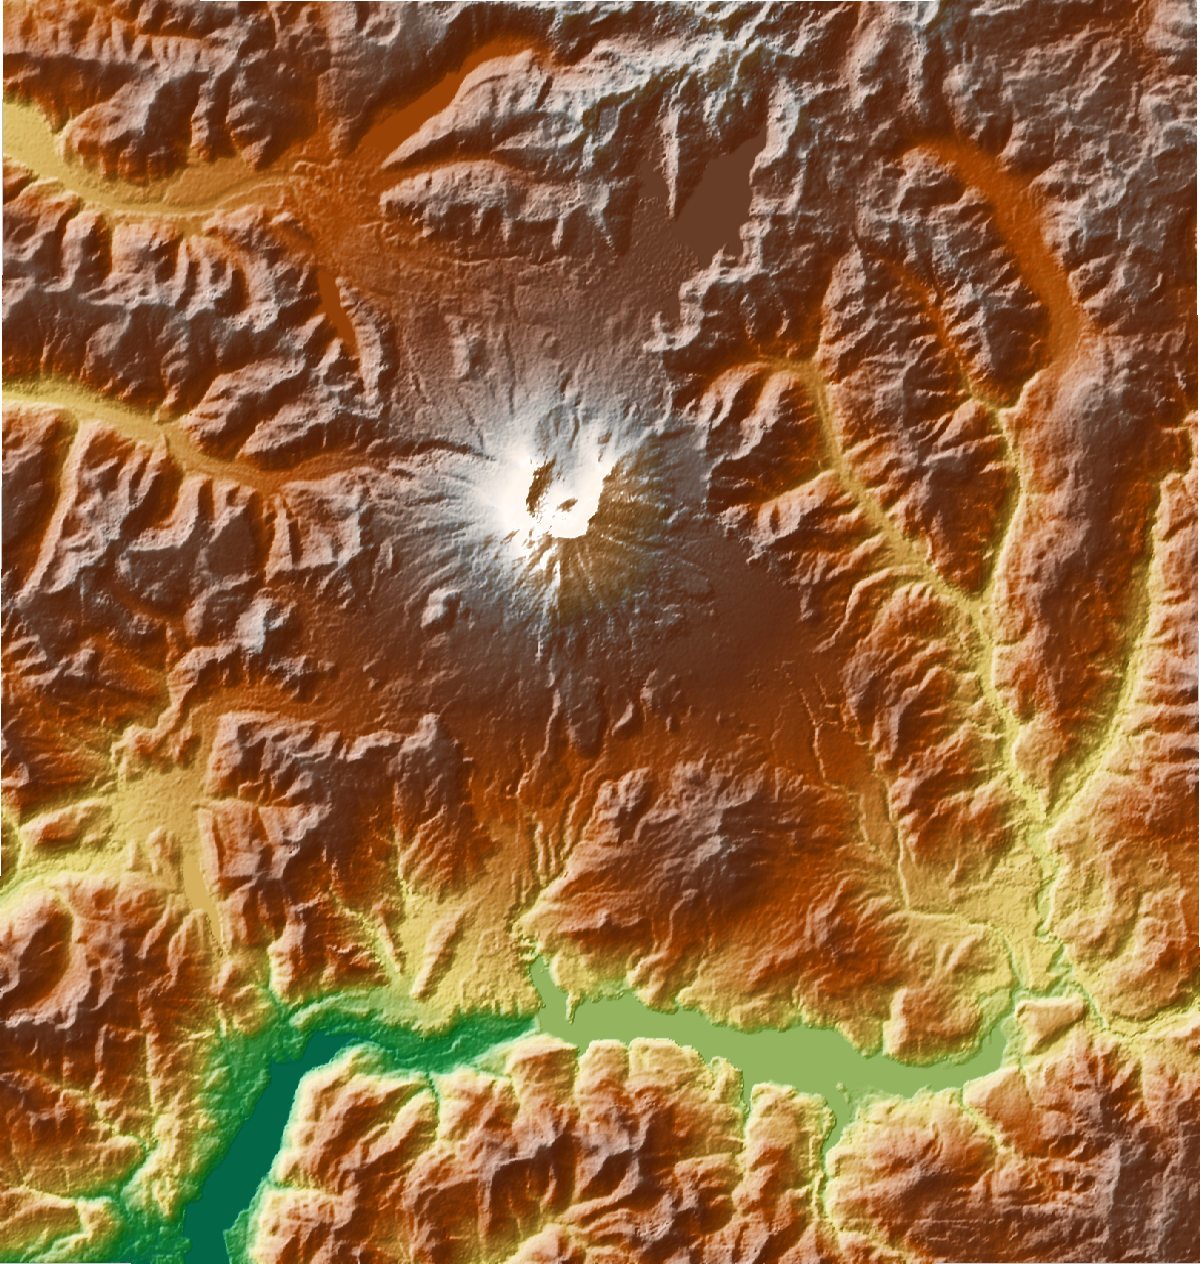
\includegraphics[width=\textwidth]{../figures/gmt_sthelens_map_01.png}
		\end{center}
	\end{columns}
\end{frame}

\begin{frame}[fragile=singleslide]
\frametitle{An example \dots Mt. St. Helens}
	\begin{columns}
		\column{0.48\textwidth}
		\tiny{
		\begin{verbatim}
#!/bin/bash

gmt begin sthelens_map png,pdf

  #add DEM, Lambert projection, 4inches wide 
  #image, default illumination
  gmt grdimage @earth_relief_01s \
        -R-122.4/-121.95/46.0/46.33 \
        -JL-122.2/46.15/46.0/46.3/4i -I+d

gmt end		
		\end{verbatim}
}
		\column{0.48\textwidth}
		\begin{center}
				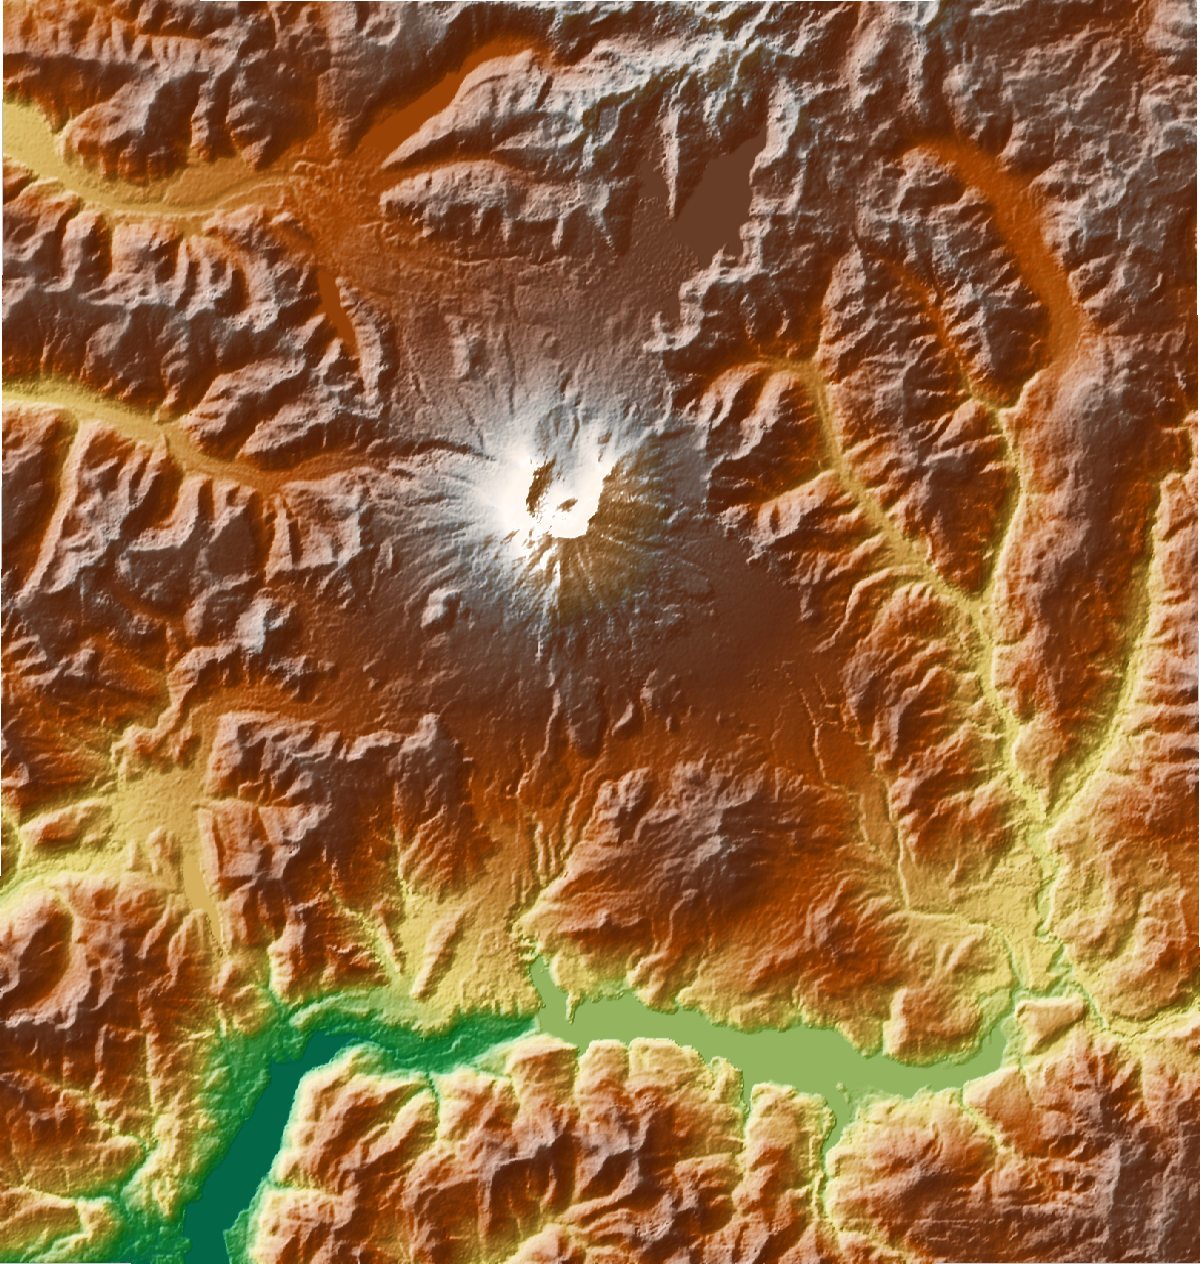
\includegraphics[width=\textwidth]{../figures/gmt_sthelens_map_01.png}
		\end{center}
	\end{columns}
\end{frame}

\begin{frame}[fragile=singleslide]
\frametitle{An example \dots Mt. St. Helens}
	\begin{columns}
		\column{0.48\textwidth}
		\tiny{
		\begin{verbatim}
#!/bin/bash

gmt begin sthelens_map png,pdf

  #add DEM, Lambert projection, 4inches wide 
  #image, default illumination
  gmt grdimage @earth_relief_01s \
        -R-122.4/-121.95/46.0/46.33 \
        -JL-122.2/46.15/46.0/46.3/4i -I+d

  #add map frame, scale bar
  gmt coast -Wthin -Ba0.1f0.01 -BWSne \
        -Lg-122.0/46.05+w5k+l+c46.1

gmt end		
		\end{verbatim}
}
		\column{0.48\textwidth}
		\begin{center}
%				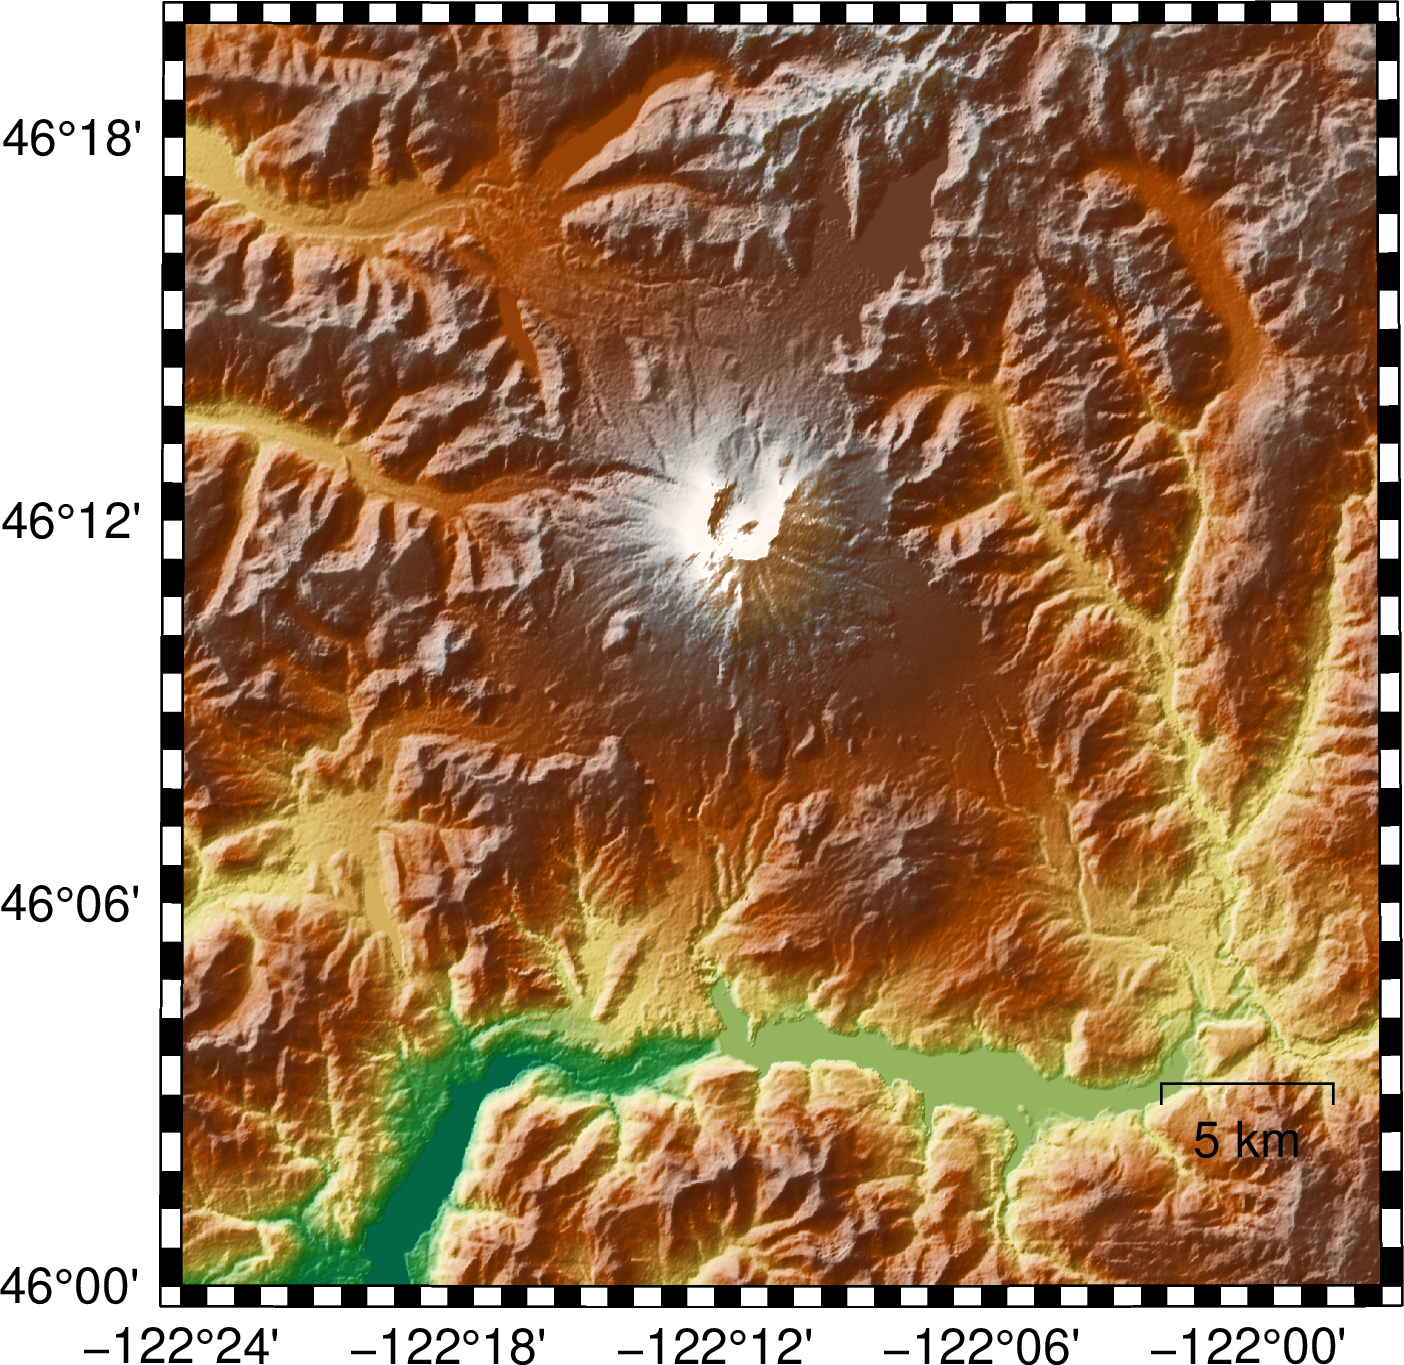
\includegraphics[width=\textwidth]{../figures/gmt_sthelens_map_02.png}	
		\end{center}
	\end{columns}
\end{frame}

\begin{frame}[fragile=singleslide]
\frametitle{An example \dots Mt. St. Helens}
	\begin{columns}
		\column{0.48\textwidth}
		\tiny{
		\begin{verbatim}
#!/bin/bash

gmt begin sthelens_map png,pdf

  #add DEM, Lambert projection, 4inches wide 
  #image, default illumination
  gmt grdimage @earth_relief_01s \
        -R-122.4/-121.95/46.0/46.33 \
        -JL-122.2/46.15/46.0/46.3/4i -I+d

  #add map frame, scale bar
  gmt coast -Wthin -Ba0.1f0.01 -BWSne \
        -Lg-122.0/46.05+w5k+l+c46.1

gmt end		
		\end{verbatim}
}
		\column{0.48\textwidth}
		\begin{center}
				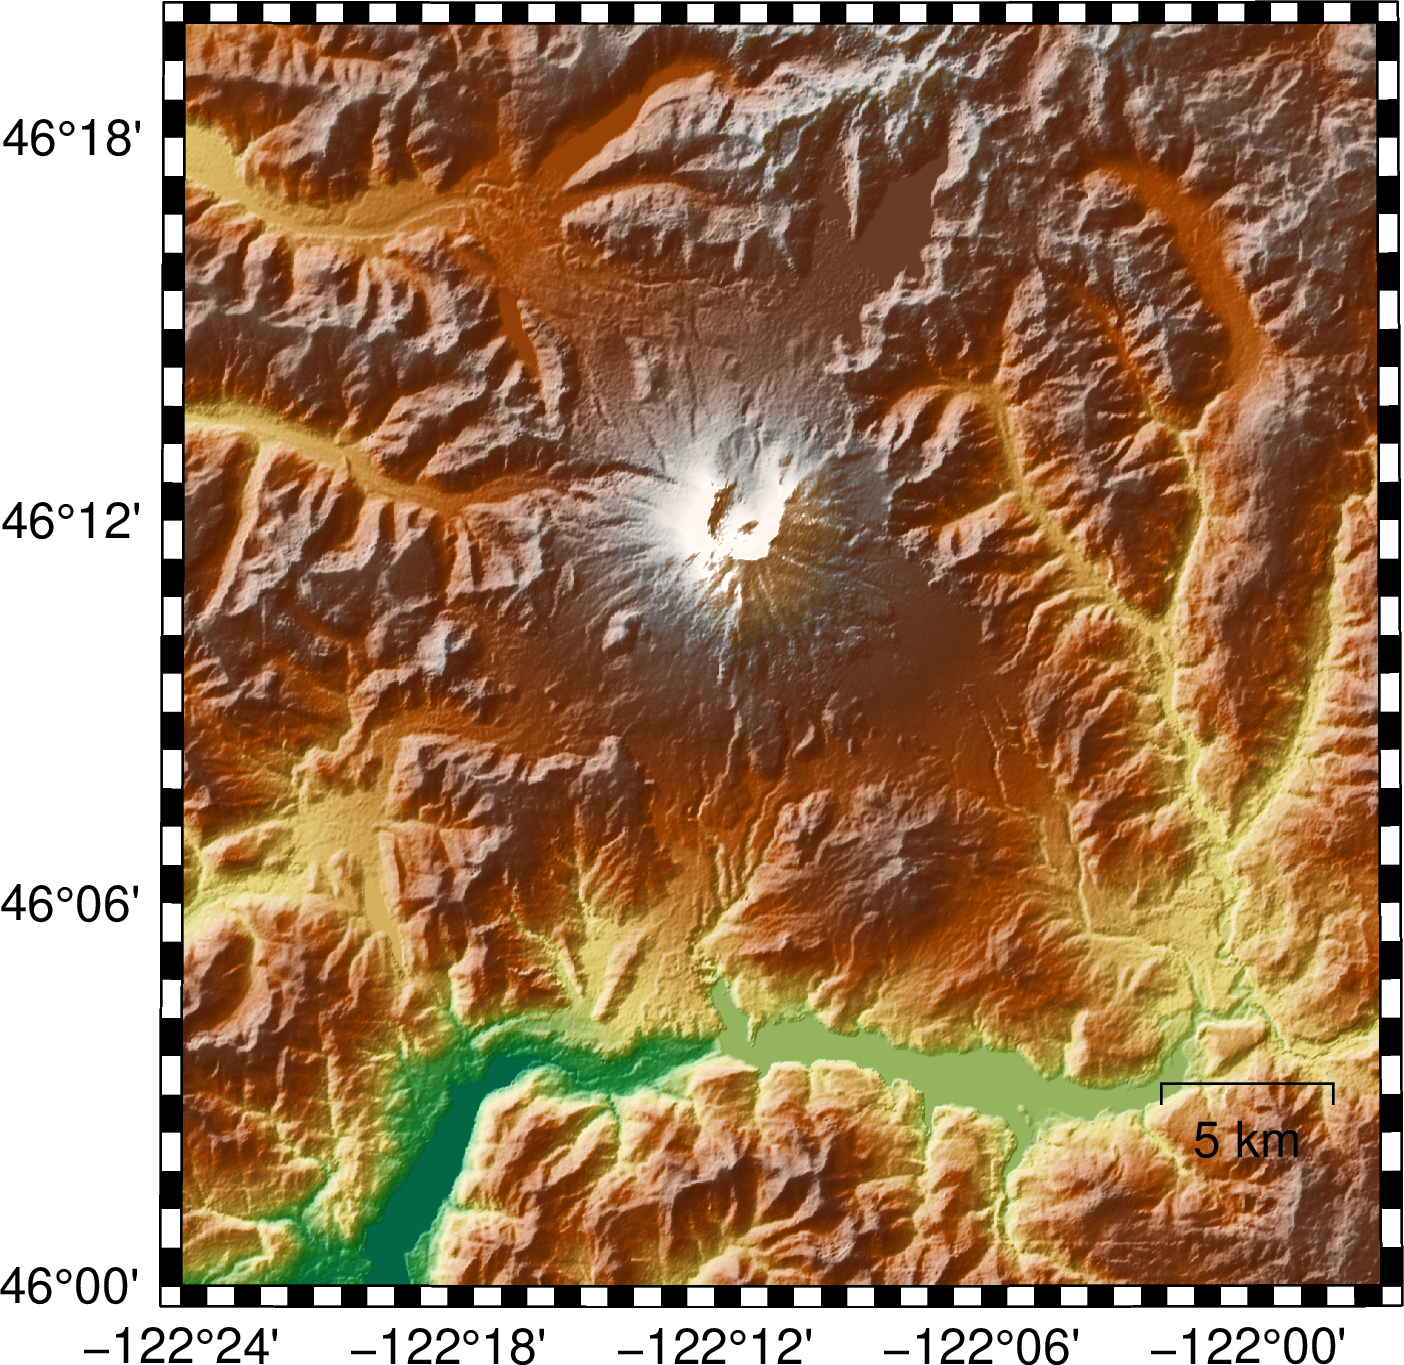
\includegraphics[width=\textwidth]{../figures/gmt_sthelens_map_02.png}	
		\end{center}
	\end{columns}
\end{frame}

\begin{frame}[fragile=singleslide]
\frametitle{An example \dots Mt. St. Helens}
	\begin{columns}
		\column{0.48\textwidth}
		\tiny{
		\begin{verbatim}
#!/bin/bash

gmt begin sthelens_map png,pdf
  #nicer map frame
  gmt set MAP_FRAME_TYPE plain

  #add DEM, Lambert projection, 4inches wide 
  #image, default illumination
  gmt grdimage @earth_relief_01s \
        -R-122.4/-121.95/46.0/46.33 \
        -JL-122.2/46.15/46.0/46.3/4i -I+d

  #add map frame, scale bar
  gmt coast -Wthin -Ba0.1f0.01 -BWSne \
        -Lg-122.0/46.05+w5k+l+c46.1

gmt end		
		\end{verbatim}
}
		\column{0.48\textwidth}
		\begin{center}
%				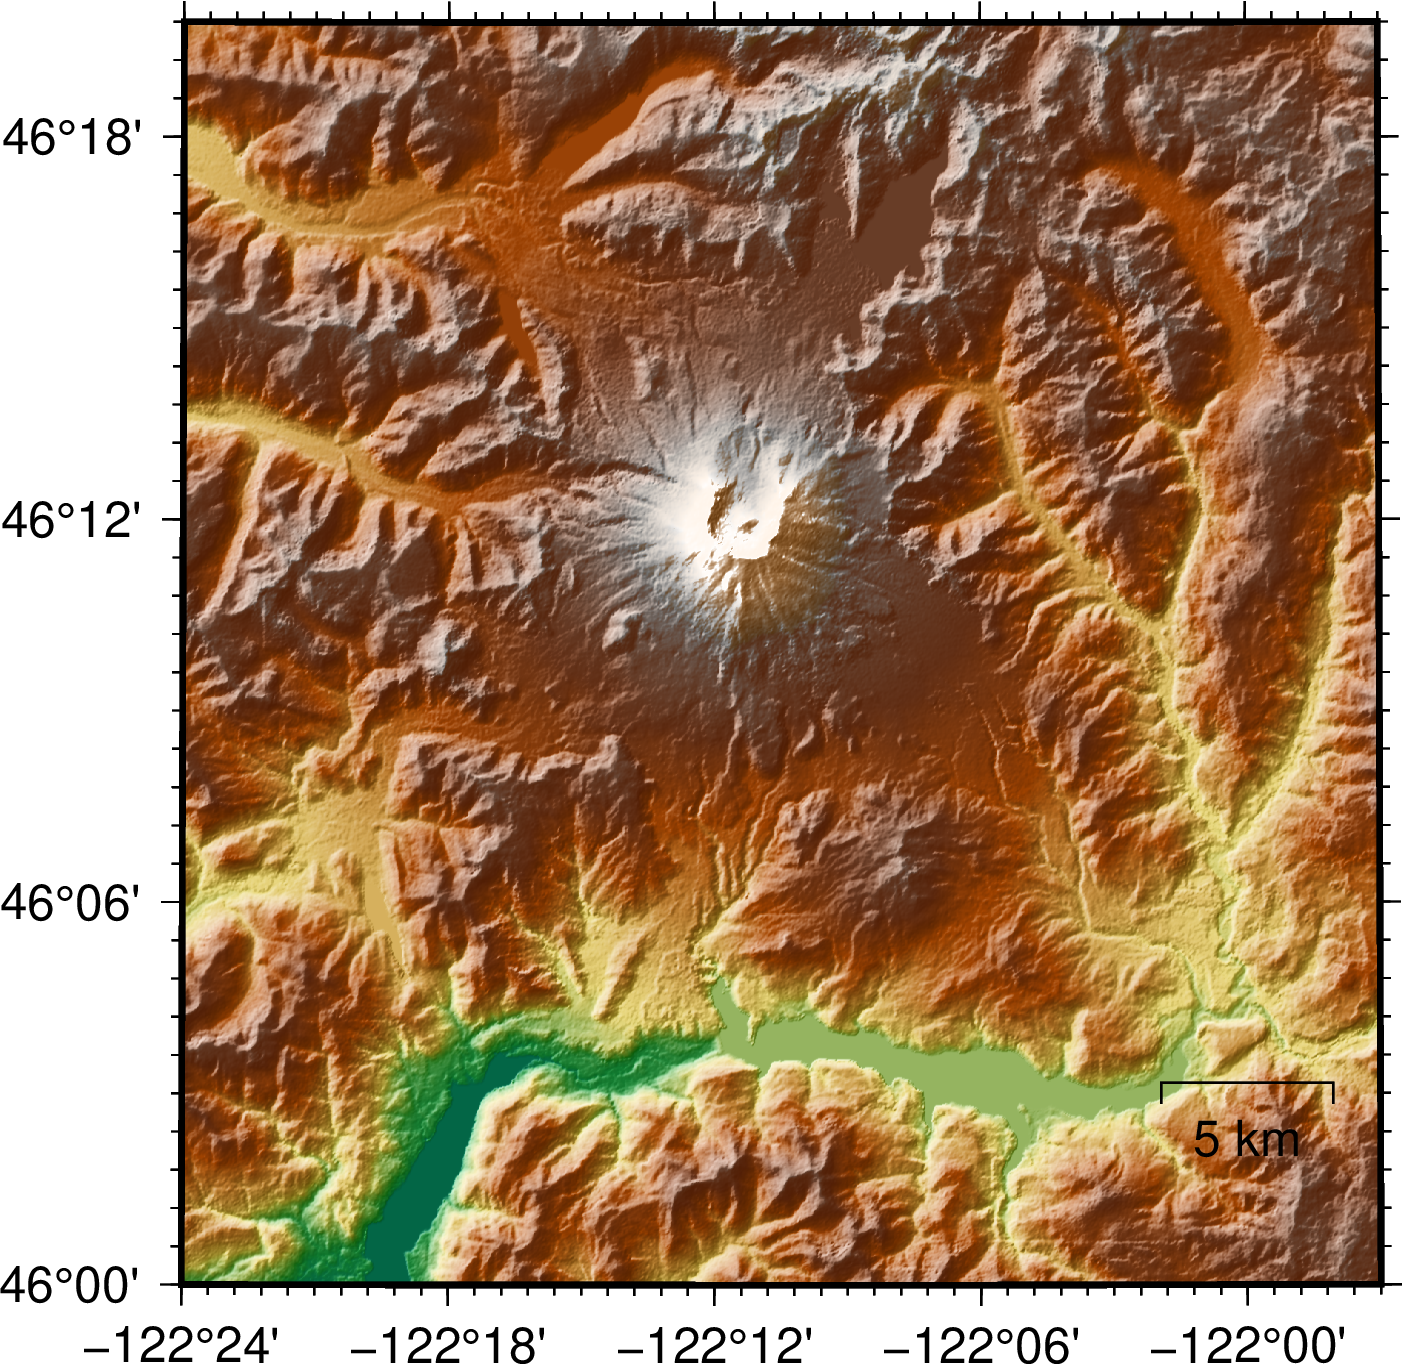
\includegraphics[width=\textwidth]{../figures/gmt_sthelens_map_03.png}	
		\end{center}
	\end{columns}
\end{frame}

\begin{frame}[fragile=singleslide]
\frametitle{An example \dots Mt. St. Helens}
	\begin{columns}
		\column{0.48\textwidth}
		\tiny{
		\begin{verbatim}
#!/bin/bash

gmt begin sthelens_map png,pdf
  #nicer map frame
  gmt set MAP_FRAME_TYPE plain

  #add DEM, Lambert projection, 4inches wide 
  #image, default illumination
  gmt grdimage @earth_relief_01s \
        -R-122.4/-121.95/46.0/46.33 \
        -JL-122.2/46.15/46.0/46.3/4i -I+d

  #add map frame, scale bar
  gmt coast -Wthin -Ba0.1f0.01 -BWSne \
        -Lg-122.0/46.05+w5k+l+c46.1

gmt end		
		\end{verbatim}
}
		\column{0.48\textwidth}
		\begin{center}
				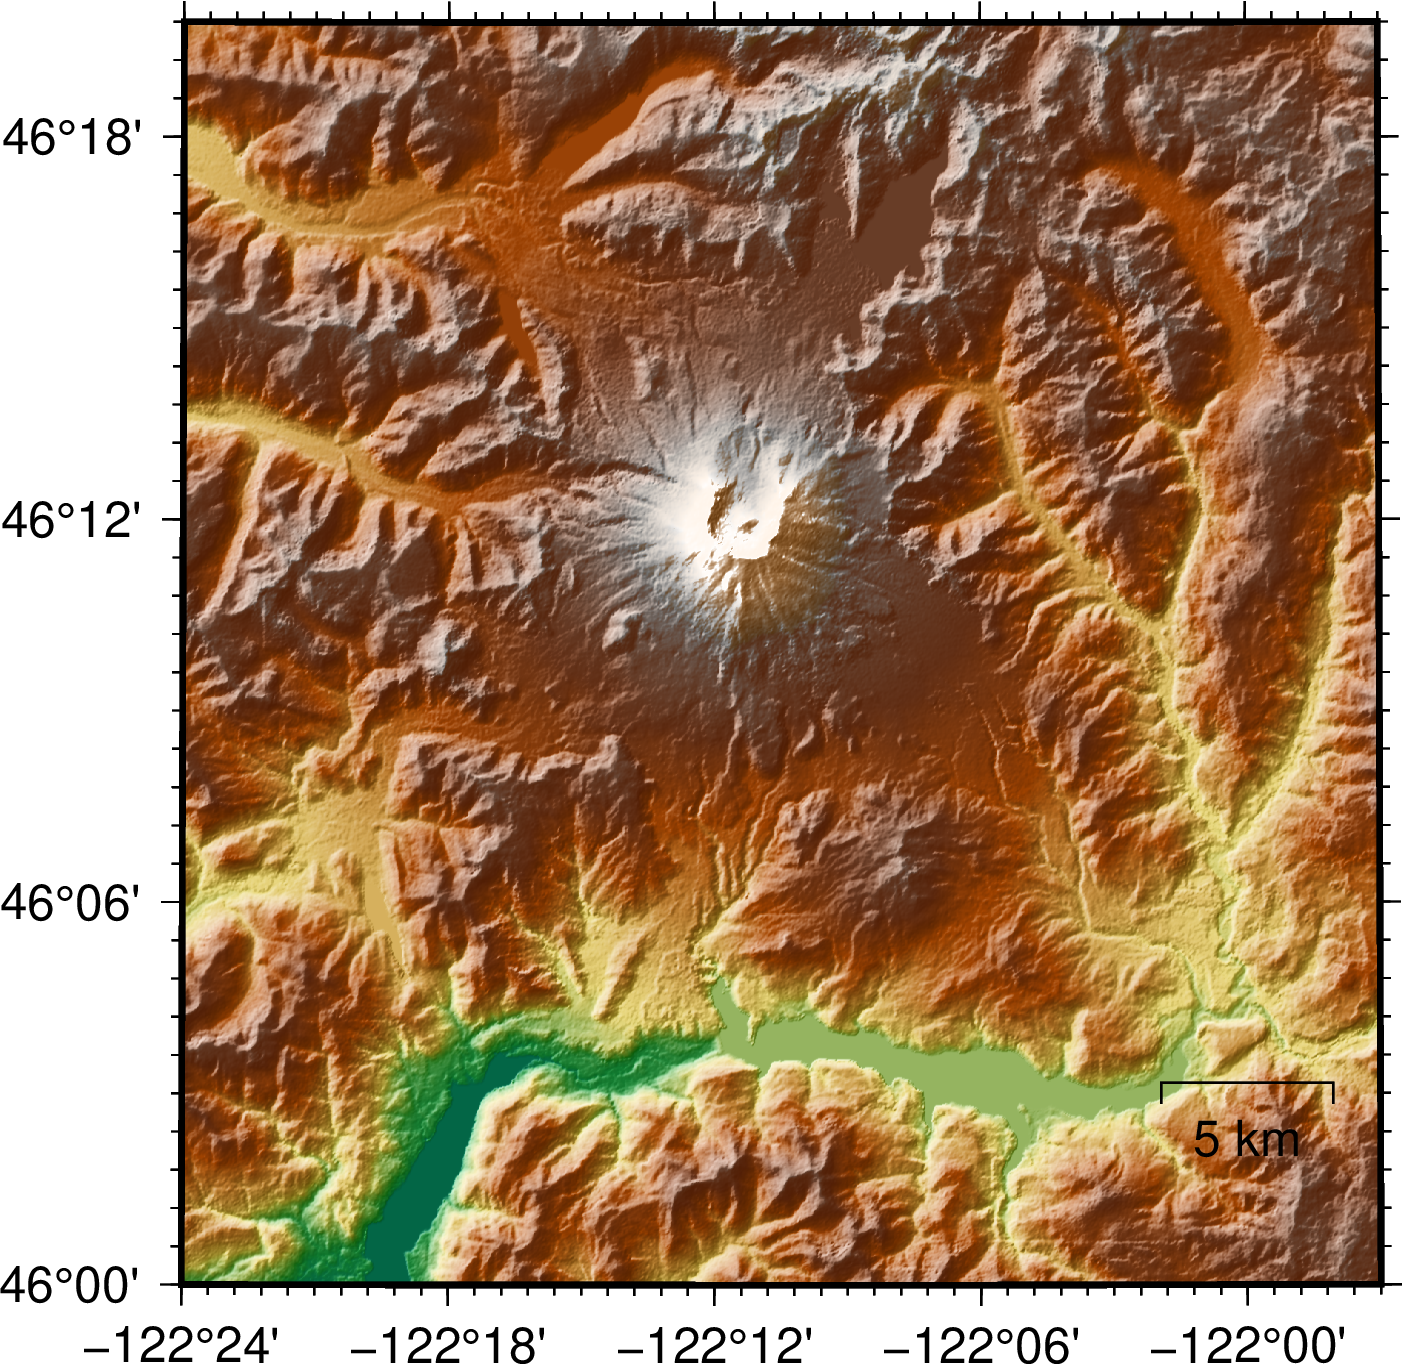
\includegraphics[width=\textwidth]{../figures/gmt_sthelens_map_03.png}	
		\end{center}
	\end{columns}
\end{frame}


\begin{frame}[fragile=singleslide]
\frametitle{An example \dots Mt. St. Helens}
	\begin{columns}
		\column{0.48\textwidth}
		\tiny{
		\begin{verbatim}
#!/bin/bash

gmt begin sthelens_map png,pdf
  #nicer map frame
  gmt set MAP_FRAME_TYPE plain

  #add DEM, Lambert projection, 4inches wide 
  #image, default illumination
  gmt grdimage @earth_relief_01s \
        -R-122.4/-121.95/46.0/46.33 \
        -JL-122.2/46.15/46.0/46.3/4i -I+d

  #add map frame, scale bar
  gmt coast -Wthin -Ba0.1f0.01 -BWSne \
        -Lg-122.0/46.05+w5k+l+c46.1

  #add GPS stations
  gmt plot -St0.2 -Gred -Wthin,red sites.xy

gmt end		
		\end{verbatim}
}
		\column{0.48\textwidth}
		\begin{center}
%				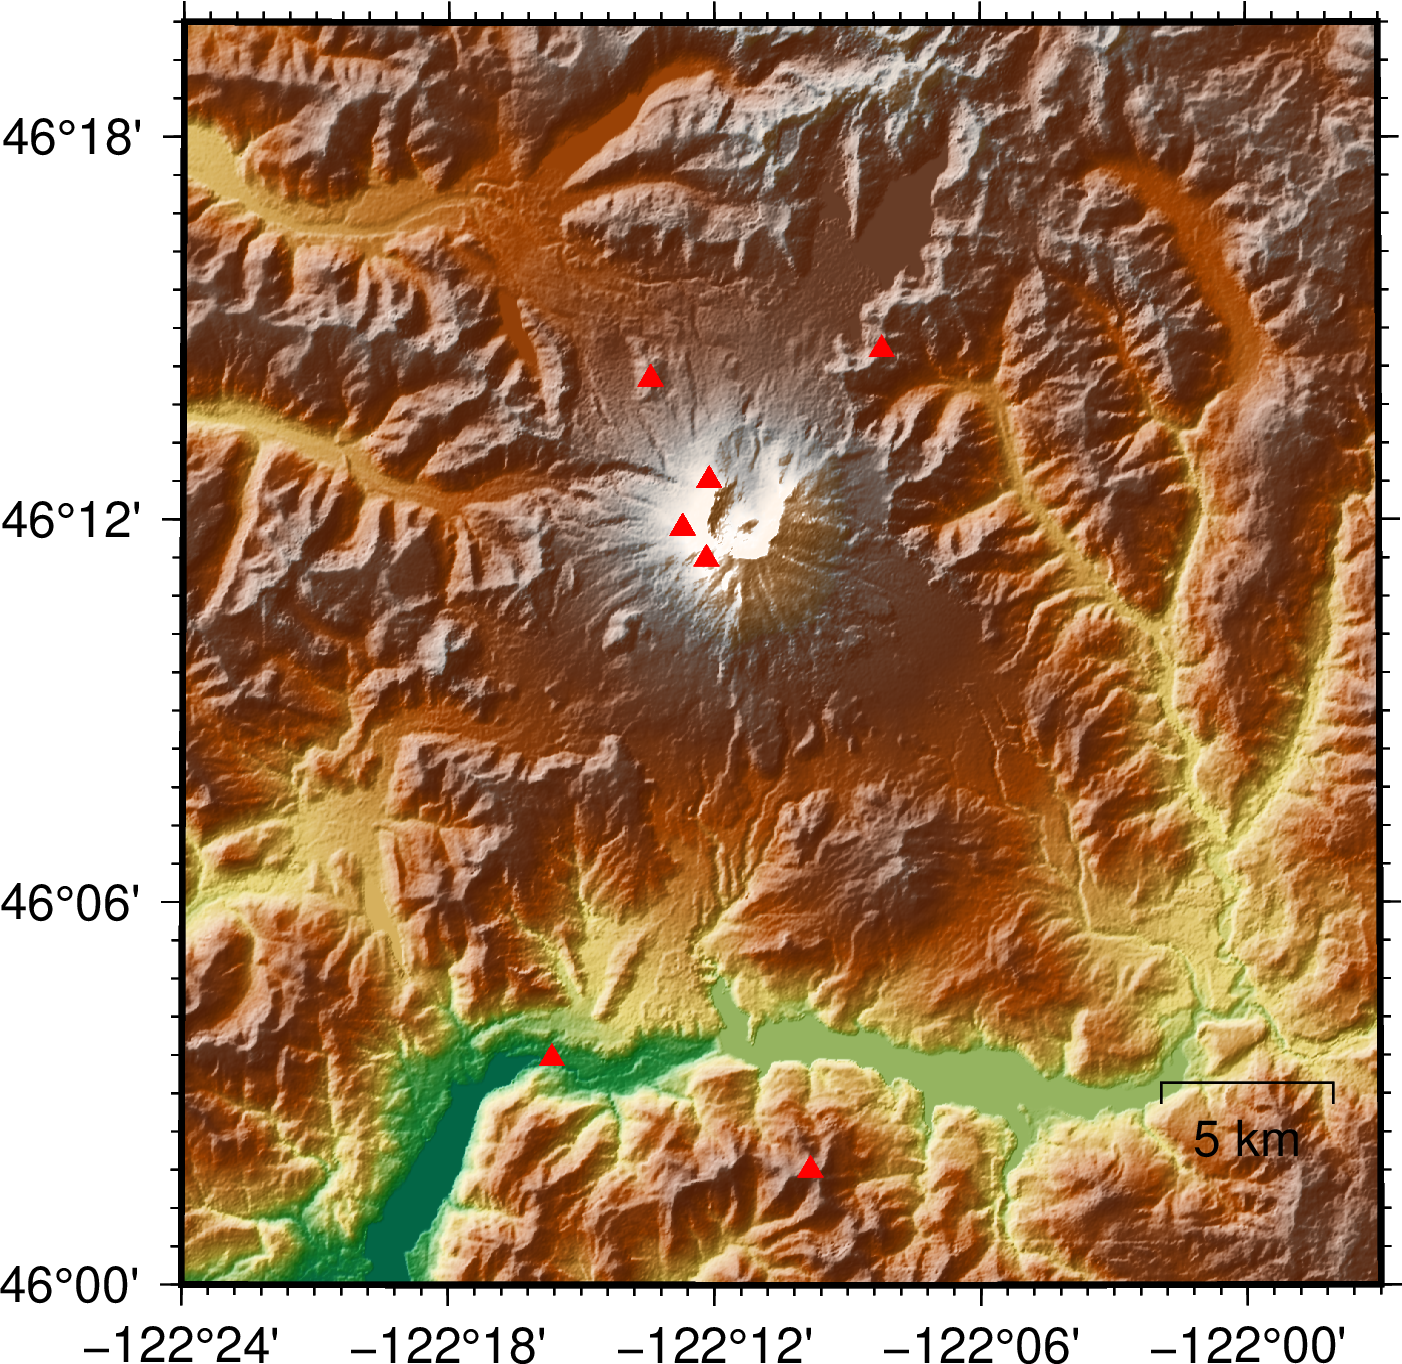
\includegraphics[width=\textwidth]{../figures/gmt_sthelens_map_04.png}	
		\end{center}
	\end{columns}
\end{frame}


\begin{frame}[fragile=singleslide]
\frametitle{An example \dots Mt. St. Helens}
	\begin{columns}
		\column{0.48\textwidth}
		\tiny{
		\begin{verbatim}
#!/bin/bash

gmt begin sthelens_map png,pdf
  #nicer map frame
  gmt set MAP_FRAME_TYPE plain

  #add DEM, Lambert projection, 4inches wide 
  #image, default illumination
  gmt grdimage @earth_relief_01s \
        -R-122.4/-121.95/46.0/46.33 \
        -JL-122.2/46.15/46.0/46.3/4i -I+d

  #add map frame, scale bar
  gmt coast -Wthin -Ba0.1f0.01 -BWSne \
        -Lg-122.0/46.05+w5k+l+c46.1

  #add GPS stations
  gmt plot -St0.2 -Gred -Wthin,red sites.xy

gmt end		
		\end{verbatim}
}
		\column{0.48\textwidth}
		\begin{center}
				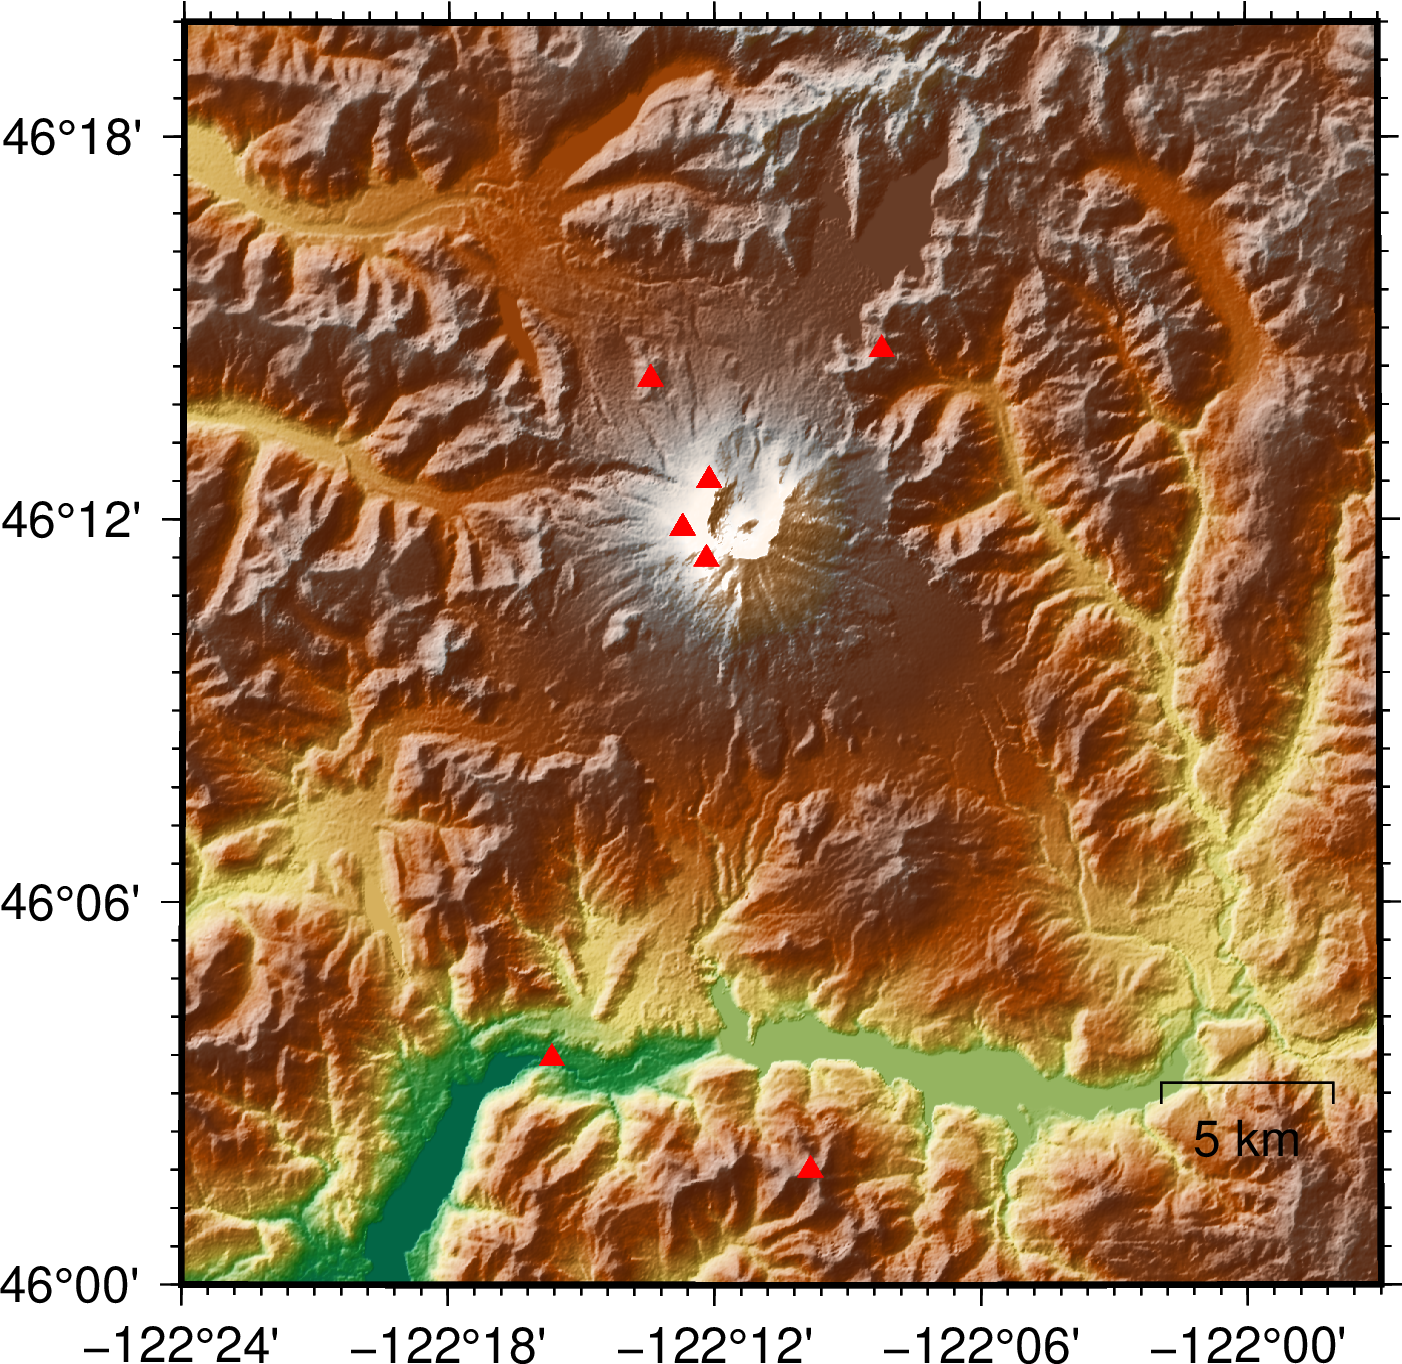
\includegraphics[width=\textwidth]{../figures/gmt_sthelens_map_04.png}	
		\end{center}
	\end{columns}
\end{frame}



\begin{frame}[fragile=singleslide]
\frametitle{An example \dots Mt. St. Helens}
	\begin{columns}
		\column{0.48\textwidth}
		\tiny{
		\begin{verbatim}
#!/bin/bash

gmt begin sthelens_map png,pdf
  #nicer map frame
  gmt set MAP_FRAME_TYPE plain

  #add DEM, Lambert projection, 4inches wide 
  #image, default illumination
  gmt grdimage @earth_relief_01s \
        -R-122.4/-121.95/46.0/46.33 \
        -JL-122.2/46.15/46.0/46.3/4i -I+d

  #add map frame, scale bar
  gmt coast -Wthin -Ba0.1f0.01 -BWSne \
        -Lg-122.0/46.05+w5k+l+c46.1

  #add GPS stations
  gmt plot -St0.2 -Gred -Wthin,red sites.xy

  #add station names
  gmt text -F+f8p,Helvetica-Bold,black+jRB \
        sites.xy
gmt end		
		\end{verbatim}
}
		\column{0.48\textwidth}
		\begin{center}
%				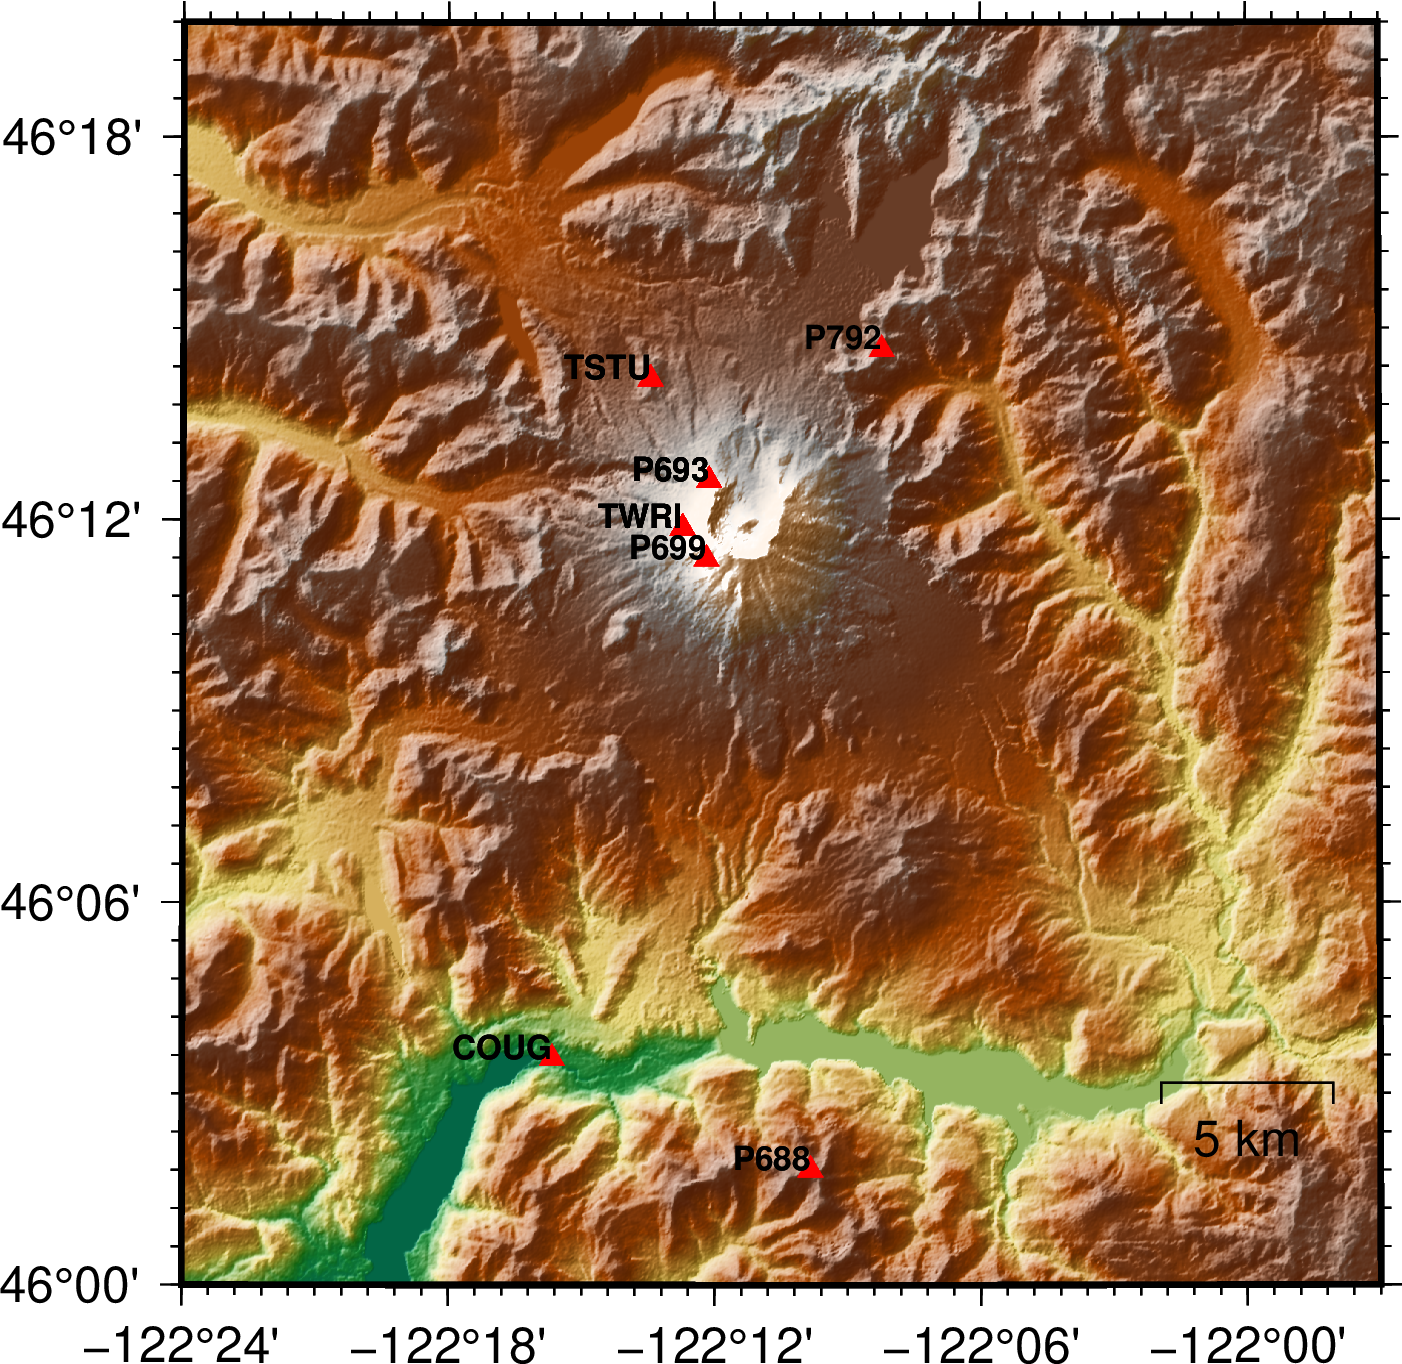
\includegraphics[width=\textwidth]{../figures/gmt_sthelens_map_05.png}	
		\end{center}
	\end{columns}
\end{frame}


\begin{frame}[fragile=singleslide]
\frametitle{An example \dots Mt. St. Helens}
	\begin{columns}
		\column{0.48\textwidth}
		\tiny{
		\begin{verbatim}
#!/bin/bash

gmt begin sthelens_map png,pdf
  #nicer map frame
  gmt set MAP_FRAME_TYPE plain

  #add DEM, Lambert projection, 4inches wide 
  #image, default illumination
  gmt grdimage @earth_relief_01s \
        -R-122.4/-121.95/46.0/46.33 \
        -JL-122.2/46.15/46.0/46.3/4i -I+d

  #add map frame, scale bar
  gmt coast -Wthin -Ba0.1f0.01 -BWSne \
        -Lg-122.0/46.05+w5k+l+c46.1

  #add GPS stations
  gmt plot -St0.2 -Gred -Wthin,red sites.xy

  #add station names
  gmt text -F+f8p,Helvetica-Bold,black+jRB \
        sites.xy
gmt end		
		\end{verbatim}
}
		\column{0.48\textwidth}
		\begin{center}
				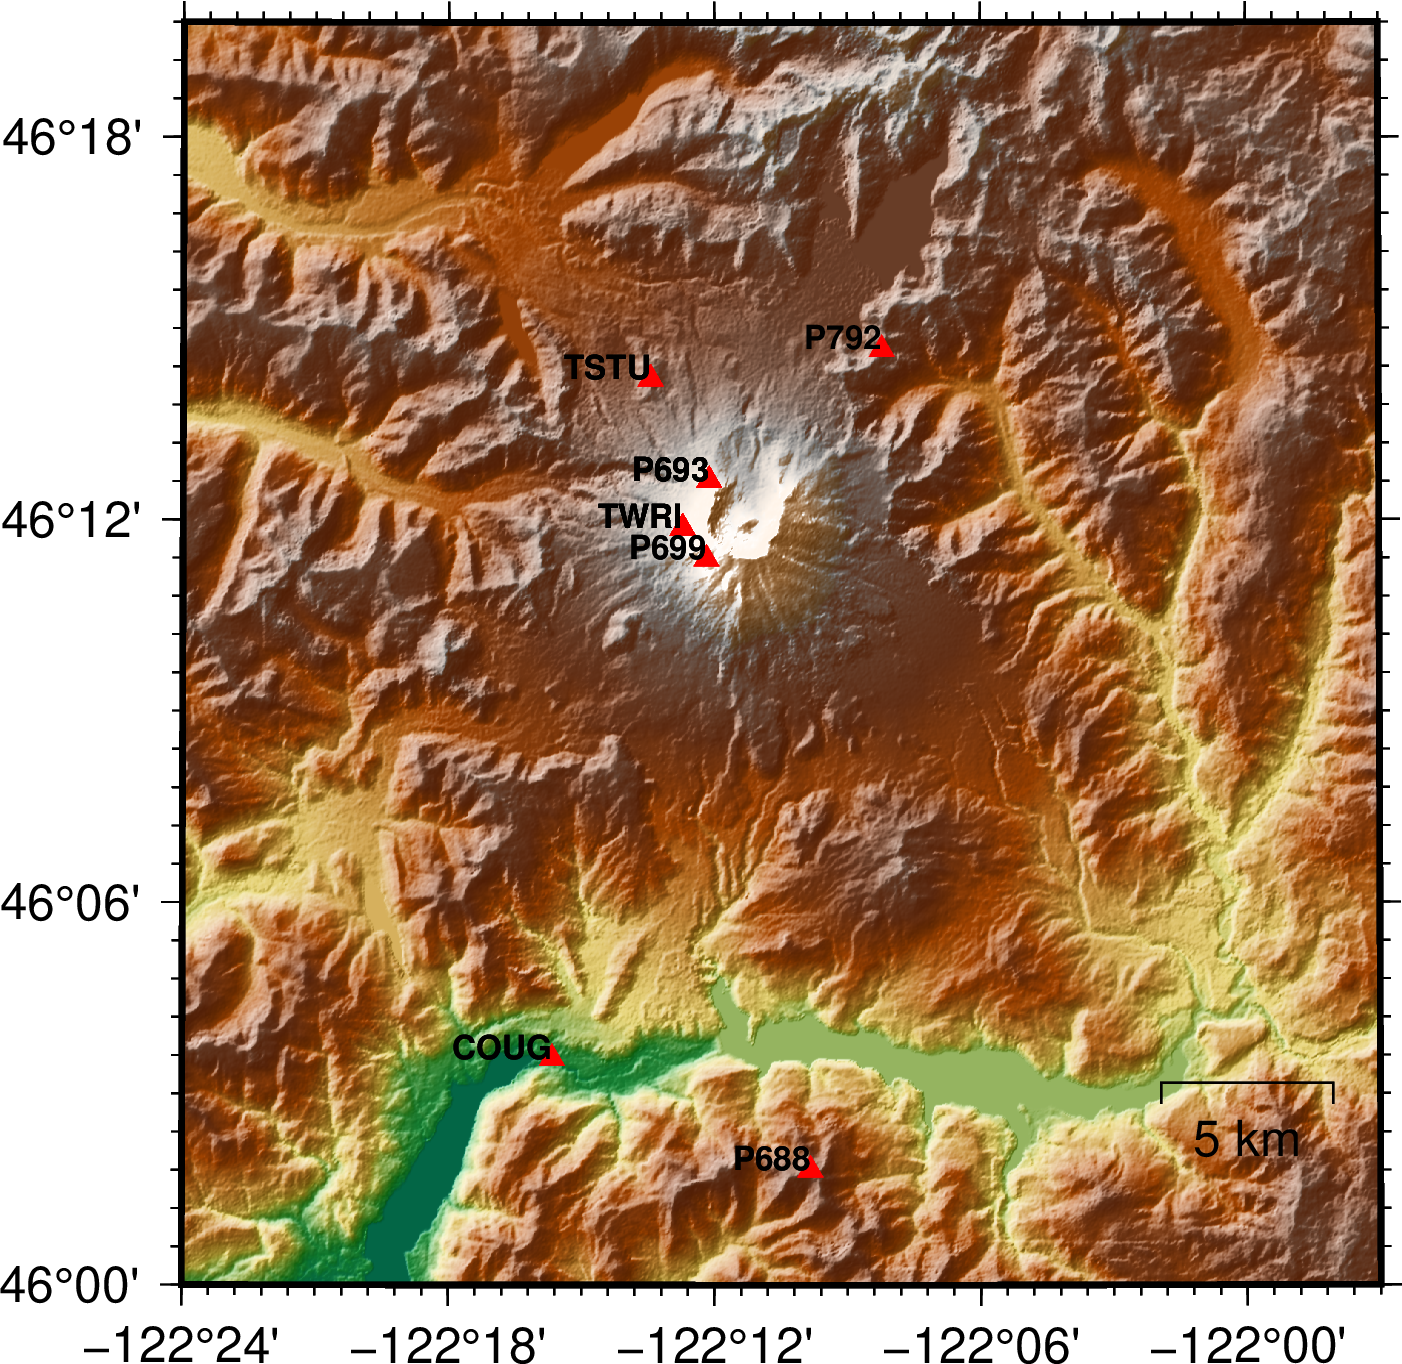
\includegraphics[width=\textwidth]{../figures/gmt_sthelens_map_05.png}	
		\end{center}
	\end{columns}
\end{frame}

\begin{frame}
\frametitle{Common Problems}
	\begin{itemize}
		\item By default: longitude first, then latitude \dots use {\tt -:} to reverse the order
		\item Definitions of some command line arguments are quite involved. (--R, --J)
		\item Read the documentation! \url{https://docs.generic-mapping-tools.org/latest/}
		\item Start from:
			\begin{itemize}
			\item Tutorial: \url{https://docs.generic-mapping-tools.org/latest/tutorial.html}
			\item Cookbook: \url{https://docs.generic-mapping-tools.org/latest/cookbook.html}
			\item Examples: \url{https://docs.generic-mapping-tools.org/latest/gallery.html}
			\end{itemize}
		\item BUILD YOUR MAPS STEP BY STEP! Don't try to do it all at once.
	\end{itemize}
\end{frame}


\end{document}
